%
% IEEE Transactions on Microwave Theory and Techniques example
% Tibault Reveyrand - http://www.microwave.fr
%
% http://www.microwave.fr/LaTeX.html
% ---------------------------------------



% ================================================
% Please HIGHLIGHT the new inputs such like this :
% Text :
%  \hl{comment}
% Aligned Eq. 
% \begin{shaded}
% \end{shaded}
% ================================================


    % This is meant to be a helpful template for papers being submitted to
% Medical Physics. It is not mandatory.
%
% Please send suggestions/improvements to drogers@physics.carleton.ca
% Sept 24, 2018
%

\documentclass[12pt]{article}   %For printing on two sides of page
					%It doesn't work with showkeys so
					%if using showkeys, use following
%\documentclass[12pt]{article}		%use with showkeys or to print one sided
\usepackage[super,sort,comma]{natbib}
\usepackage{amssymb}

%\usepackage[super,sort&compress,comma]{natbib}
% use the version without compress to get everything working. Then on ONE,
% and ONLY ONE FINAL RUN, use the version with compress to change 1,2,3,4
% to 1-4 etc in the citations.  Otherwise hyperref gets confused.


\usepackage{fancyhdr}		%Gives headers and footers defined below
\renewcommand{\footrulewidth}{0.4pt} %thickness of line above footer

%\usepackage{showkeys}		%may use for drafting
				%comment out for final submission

%The following is useful for creating captions for figures and tables that have
%a different font and different width on the page. This separates them from
%text.
\newcommand{\captionv}[3]{\begin{center}\parbox{#1cm}{\caption[#2]{{\sf #3}}}
        \end{center}}
	%use as   \captionv{N}{B}{C}
	%first entry,N, is width of caption in cm
	%second entry, B, is a short title that appears in list of figure/tables
	%     B can be blank. The lists are not needed
	%third entry, C, is the caption for the figure or the table
	%    Note that the \label{fig_text} should be part of entry C.

\usepackage[section]{placeins}   %
%above package forces all floats (tables figures) to be processed before a
%new section starts. Unlike using \clearpage, this will start the section
%on the same page as the float, but after it.
%might not work with subsections, but if that is the case, put
%  \FloatBarrier just before the \subsection

\usepackage{graphicx}
\usepackage{hyperref}
\usepackage{url}

%following lines fix up style of bibliography to be superscripts
\makeatletter \renewcommand\@biblabel[1]{$^{#1}$} \makeatother
 \setlength{\bibhang}{0em}
 \setlength{\labelsep}{1em}     
 \setlength{\itemindent}{-\bibhang}
 \setlength{\leftmargin}{\bibhang}


%set dimensions of the page for 8.5x11 inch paper
\setlength{\textwidth}{16.5cm}
\setlength{\headwidth}{16cm}		%for fancy page style only
\setlength{\textheight}{22.6cm} 
\setlength{\oddsidemargin}{-1mm}
\setlength{\evensidemargin}{-2mm} 
\setlength{\topmargin}{-1.0cm}

\setlength{\parindent}{2em}   %indent paragraph 2 letters m
\setlength{\parskip}{1.3ex}   %paragraph break
\setlength{\floatsep}{20pt}
\setlength{\textfloatsep}{20pt}		%space below a figure/table def 20pt
\setlength{\intextsep}{20pt}		%space below a figure/table def 20pt
					%p142 compendium

%Following is for Med Phys numbering  I.A.1  etc
\renewcommand{\thesection}{{\sf \Roman{section}}.}
\renewcommand{\thesubsection}{\thesection{\sf \Alph{subsection}}.}
\renewcommand{\thesubsubsection}{\thesubsection{\sf \arabic{subsubsection}}.}
\renewcommand{\theparagraph}{\alph{paragraph}.}


% following is useful during drafting when you want to flag something for
% other authors or for yourself. It can be used throughout the text.
\newcommand{\note}[1]{\mbox{}\\ \noindent \rule{16cm}{0.5mm} \\
{\em #1} \\ \noindent \rule{16cm}{0.5mm}
\typeout{    }
\typeout{*note active on this page *}
\typeout{Note: #1  }
\typeout{end Note}
}

% Uncomment the following to remove all notes from the paper
% \renewcommand{\note}[1]{}


% These can be used to identify where a figure or table is first referenced 
% by placing a margin note.  If the figures/tables are inserted in the text
% they are not needed.

\newcommand{\mfig}[1]{\marginpar{{\sf Fig~\ref{#1} }}}
\newcommand{\mtab}[1]{\marginpar{{\sf Table~\ref{#1} }}}

%Following are just useful shortcuts and not mandatory
\newcommand{\cen}[1]{\begin{center} #1 \end{center}}
\newcommand{\eqn}[1]{\begin{equation} #1 \end{equation} }

%The following allow lists to be more compact than the default. Not
%mandatory, but useful.
\newenvironment{packed_enum}{
\begin{enumerate}
  \setlength{\itemsep}{1pt}
  \setlength{\parskip}{0pt}
  \setlength{\parsep}{0pt}
}{\end{enumerate}}

\newenvironment{packed_item}{
\begin{itemize}
  \setlength{\itemsep}{1pt}
  \setlength{\parskip}{0pt}
  \setlength{\parsep}{0pt}
}{\end{itemize}}

\renewcommand{\refname}{}       %













% The following only needed if you use the headers/footers. Not essential
% but can be useful      

% [on even pages]{on odd pages} %even pages only active f using twosided
				%if no even given, uses same for both
% lhead is left head, etc
%\lhead[{\sffamily page~\thepage}]{{\sffamily  Running title here: Printed \today}}
% the $Date:$ below is replaced by the date the file was last edited when using
% CVS.  If not being used, comment this out.
%\lfoot[{\sf \leftmark}]{{\small {\sf Last edited $Date:$ }}}
%\rhead[{\sf 1st author name or however authors to be briefly identified}]{{\sf page~\thepage}}
%\rfoot[{\sffamily {\rightmark}}]{{\sffamily {\rightmark}}}
%\cfoot{}
%\chead{}


% the following is used to suppress many warnings that don't effect the
% output 
\typeout{*Have turned off overfull and underfull messages}
\tolerance=10000        %suppress Overfull only
\hbadness=10000         %suppress Overfull and Underfull for text (horizontal)
\vbadness=10000         %suppress Overfull and Underfull for vertical "boxes"

% Now set up for line numbers.  If the files lineno.sty is not on the latex
% path, the following assumes it is on the area the .tex file is located.

% Select the way you prefer line numbers by uncommenting the way you prefer.
% I prefer continuous line numbers but don't need them for tables.

% \usepackage[pagewise,mathlines,edtable]{lineno}
% \usepackage[mathlines,edtable]{lineno}
\usepackage[mathlines]{lineno}
%  pagewise => start new line number each page. Otherwise number from start
%  edtable => line num for table. Needs \begin{edtable}{tabular}{|c|}   etc
%                        and \end{edtable}  We don't need \end{tabular}

% \linenumbers
% \modulolinenumbers[5]
% Comment out the above line and all line numbers are removed EXCEPT in
% tables.   To get rid of those you need to remove edtable at the start and
% stop of the table.

%%%%%%%%%%%%%%%%%%%%%%%%%%%%%%%%%%%%%%%%%%%%%%%%%%%%%%%%%%%%%%%%%%%%%%%%%%%%%%%
%               set up hyperref for the pdf outputs
%  This makes all references linked to tables, references etc
%%%%%%%%%%%%%%%%%%%%%%%%%%%%%%%%%%%%%%%%%%%%%%%%%%%%%%%%%%%%%%%%%%%%%%%%%%%%%%%
%

\usepackage{hyperref}
\hypersetup{colorlinks,
    citecolor=blue,
    filecolor=blue,
    linkcolor=blue,
    urlcolor=blue
}
\usepackage[font=scriptsize]{caption}
\usepackage{subcaption}
% if lines down to % end \backrefalt are uncommented, => in reference list there
% will be pointers to where the references are used. Useful in drafting
% but should be commented out for submission.
%\usepackage[pagebackref]{hyperref}
%\renewcommand*{\backref}[1]{}
%\renewcommand*{\backrefalt}[4]{%
%  \ifcase #1 %
%    \relax%No citations.% use \relax if do not want the "No citations" message
%  \or
%    (p #2)%
%  \else
%    (pp #2)%
%  \fi%
%}
% end \backrefalt   Always leave this line commented out

% some more options. Just use one hyperref option at a time
%\usepackage[dvipdfm]{hyperref}  %if using latex producing .dvi rather than .pdf
%\usepackage[dvipdfm,pagebackref]{hyperref} %version will show page number
          %that a reference is cited on. Useful for checking they are all used.
\usepackage{color} 
\usepackage{graphicx}
\usepackage[table,dvipsnames]{xcolor}

\usepackage{array}
\usepackage{mdwmath}
\usepackage{mdwtab}
\usepackage{eqparbox}
\usepackage{url}
\usepackage{amsmath}
\usepackage{hyperref}
\usepackage{caption}
\usepackage{subcaption}
\usepackage{tikz}
\usepackage{pgfplots}
\usetikzlibrary{spy,calc}
\usetikzlibrary{backgrounds}
\usetikzlibrary{decorations}
\usepackage{multirow}
\renewcommand{\thesubfigure}{\roman{subfigure}}
\usepackage{adjustbox}
\usepackage{ulem}
\renewcommand{\thefootnote}{\textcolor{black}{\roman{footnote}}}
\usepackage{float}
\usepackage{algorithm}
\usepackage{algorithmic}

\usepackage[table,dvipsnames]{xcolor}
        %\textcolor{declared-color}{text}    OR   {\color   text}
        %The difference between \textcolor and \color is the same as that
        %between \texttt and \ttfamily, you can use the one you prefer. The
        %\color environment allows the text to run over multiple lines and
        %other text environments whereas the text in \textcolor must all be
        %one paragraph and not contain other environments.

        %\colorbox{declared-color}{text}   will change background color
\definecolor{gray}{rgb}{0.6,0.6,0.6}
\definecolor{red}{rgb}{0.85,0,0}
\definecolor{green}{rgb}{0,0.85,0}
\definecolor{blue}{rgb}{0,0,0.85}
\definecolor{beige}{rgb}{0.92,0.87,0.78}
%%%%%%%%%%%%%%%%%%%%%%%%%%%%%%%%%%%%%%%%%%%%%%%%%%%%%%%%%%%%%%%%%%%%%%%%%%%%%%%
\usepackage[all]{hypcap}    %causes link to figures to go to figure, not caption
%%%%%%%%%%%%%%%%%%%%%%%%%%%%%%%%%%%%%%%%%%%%%%%%%%%%%%%%%%%%%%%%%%%%%%%%%%%%%%%

\DeclareMathOperator*{\argmin}{argmin} % no space,

%%%%%%%%%%%%%%%%%%%%%%%%%%%%%%%%%%%%%%%%%%%%
\usepackage{etoolbox}

\makeatletter % <=======================================================
\let\myorg@bibitem\bibitem
\def\bibitem#1#2\par{%
  \@ifundefined{bibitem@#1}{%
    \myorg@bibitem{#1}#2\par
  }{%
    \begingroup
      \color{\csname bibitem@#1\endcsname}%
      \myorg@bibitem{#1}#2\par
    \endgroup
  }%
}
% \newcommand*{\bibitem@dp}{black}    % <==================
% \newcommand*{\bibitem@th}{black}  % <==================
% \newcommand*{\bibitem@washin}{black}  % <==================
% \newcommand*{\bibitem@washout}{black}  % <==================
% \newcommand*{\bibitem@SER}{black}  % <==================
% \newcommand*{\bibitem@larsson}{black}  % <==================
% \newcommand*{\bibitem@brix}{black}  % <==================
% \newcommand*{\bibitem@tofts}{black}  % <==================
% \newcommand*{\bibitem@etofts}{black}  % <==================
% \newcommand*{\bibitem@vsidak}{black}  % <==================
% \newcommand*{\bibitem@sidak}{black}  % <==================
% \newcommand*{\bibitem@twocxm}{black}  % <==================
% \newcommand*{\bibitem@paldinofundamentals}{black}  % <==================
% \newcommand*{\bibitem@kettelkamparterial}{black}  % <==================
% \newcommand*{\bibitem@bliesenerefficient}{black}  % <==================
% \newcommand*{\bibitem@breastdatatwopaper}{black}  % <==================
% \newcommand*{\bibitem@QINbreasttwo}{black}  % <==================
% \newcommand*{\bibitem@americanacr}{black}  % <==================

%\newcommand*{\bibitem@brix}{black}  % <==================

%\newcommand*{\bibitem@A1}{red}      % <================== error A1
\makeatother % <========================================================


\linenumbers
\modulolinenumbers[1]

\pagenumbering{arabic}
%%%%%%%%%%%%%%%%%%%%%%%%%%%%%%%%%%%%%%%%%%%%%
\begin{document}

\begin{center}
{\ } 

{\Large\bf Performance Benchmarking of Deep Learning Models for Real-Time Median Nerve Segmentation and Cross-Sectional Area Measurement in Ultrasound Imaging}
{\ }\\ 
{\ }\\
{\ }\\

 \large{Vaddadi Venkatesh$^{}$$^{1}$}, \large{Lokesh Bathala$^{}$$^{2}$}, \large{Raji Susan Mathew$^{}$$^{3}$}, and \large{Phaneendra K. Yalavarthy, $^{\ast,}$$^{1}$}\\
\noindent
{$^{1}$ Department of Computational and Data Sciences, Indian Institute of Science, Bangalore- 560012 India}\\
{$^{2}$ Aster CMI Hospital, Hebbal, Bangalore- 560092, India }\\
{$^{3}$ School of Data Science, Indian Institute of Science Education and Research, Thiruvananthapuram- 695551, India}\\
% \email
{$^\ast$e-mail: yalavarthy@iisc.ac.in}\\
{\textit{RUNNING TITLE}: \hspace{0.2cm} MNSeg-Net for Median Nerve Segmentation in Ultrasonography }\\
{\ }
{\ }\\
{\ }\\
{\ }\\
 {\ } \\
 {\ } \\
 {\ }\\
{\ }\\
{\ }\\
 {\ } \\
 {\ } \\
  {\ } \\
 {\ } \\
{\ }\\
 {\ } \\
 {\ } \\
 {\ }\\
{\ }\\
{\ }\\
 {\ } \\
 {\ } \\
  {\ } \\
 {\ } \\
\emph{Medical Physics}\\
Submitted on: \today\\
\end{center}
\newpage
\begin{abstract}  
\noindent \textbf{Background:} Median nerve, a major peripheral nerve, connects the hand to the central nervous system, facilitating upper limb motor function and sensation by transmitting sensory data from the palm and fingers. Damage to this nerve can result in motor and sensory deficits, with carpal tunnel syndrome (CTS) causing compression, leading to tingling and numbness in the thumb, index, middle, and lateral ring fingers.

\noindent \textbf{Purpose:}  This study aimed to develop an accurate deep-learning-based segmentation method for measuring the cross-sectional area (CSA) of the median nerve to facilitate the diagnosis of nerve entrapment syndromes and aid in surgical planning, with a focus on CTS.


\noindent \textbf{Methods:} This study introduces MNSeg-Net, a novel lightweight multiscale feature fusion network with 2.46M parameters for median nerve segmentation in ultrasound (US) frames, specifically designed to enable a fully automated, end-to-end clinical setup supporting real-time segmentation and CSA computation. The dataset comprised 100 subjects and 30,000 ultrasound frames, which were split into training (80\%), validation (10\%), and testing (10\%) subsets with subject-wise separation to avoid data leakage. MNSeg-Net was benchmarked against state-of-the-art segmentation models, including UNet and its variants (UNet++ and U2Net). The performance was assessed using metrics such as the Dice Similarity Coefficient (DSC) and CSA difference. The statistical significance of performance differences was evaluated using paired t-tests, effect size (Cohen’s d), and one-way ANOVA with Tukey’s HSD correction for multiple comparisons at a $p$-value threshold of 0.05, while statistical equivalence between models within predefined margins was formally assessed using the two one-sided test (TOST) procedure. Following quantitative validation, the model was deployed in a real-time clinical setup utilizing an Av.io HD Epiphan frame grabber to stream ultrasound images from the ultrasound machine to a GPU-equipped system. A secondary display running parallel to the original ultrasound screen visualized the segmented median nerve and computed the CSA values in real time.


\noindent \textbf{Results:}  
MNSeg-Net achieved high segmentation performance, with average DSC scores of 94.7\% at the wrist and 83.4\% from the wrist to the elbow, and the lowest Hausdorff distance, matching the performance of the best-performing 44-million-parameter heavy U2Net model. Compared to U2Net, MNSeg-Net showed no statistically significant difference in DSC performance ($p = 9.11 \times 10^{-1}$; Cohen’s $d = -0.003$; mean difference = –0.001), with formal equivalence testing confirming equivalence across all tested margins ($\pm0.01, \pm0.03, \pm0.05$). For CSA estimation, MNSeg-Net also showed no statistically significant difference from clinician-annotated values ( $p = 1.14 \times 10^{-1}$; Cohen’s $d = -0.041$; mean difference = –0.081), and equivalence was established at the $\pm0.5$ margin, confirming a strong alignment with expert clinical assessments. MNSeg-Net demonstrated real-time performance by processing up to 43 frames per second on a single GPU, successfully segmenting the median nerve and computing CSA from ultrasound frames.


\noindent
\textbf{Conclusion:} The developed MNSeg-Net–based clinical system represents an important step toward real-time median nerve assessment, enabling a fully automated solution for CTS diagnosis. By combining a lightweight architecture, real-time processing capability, and successful clinical deployment, it represents a substantial advancement in the CTS detection and management.

\end{abstract}
\noindent {{\bf Keywords:} Median Nerve Segmentation, Ultrasound Video, Lightweight Network, Real-time Clinical Setup.}

% ====================================================================
% ====================================================================
% ====================================================================


%\newpage


\section{Introduction}
The median nerve is a major peripheral nerve that serves as a critical communication pathway between the hand and central nervous system and is crucial for upper limb motor function and sensation \cite{soubeyrand2020anatomy,agarwal2014cadaveric,henry2015prevalence}. It transmits sensory data from the palms and fingers to the central nervous system, which is essential for touch, temperature, and pain perception. Damage to the median nerve can result in notable impairment of movement and sensation. Carpal tunnel syndrome (CTS)\cite{soubeyrand2020anatomy,ehler2017median}, the most common peripheral neuropathy, affects the thumb, index finger, middle finger, and the lateral side of the ring finger. It typically arises because of increased pressure within the enclosed carpal tunnel, which compresses the median nerve and is characterized by tingling and numbness in the affected hand.
\begin{figure} [htbp]
    \centering
      \scalebox{1}{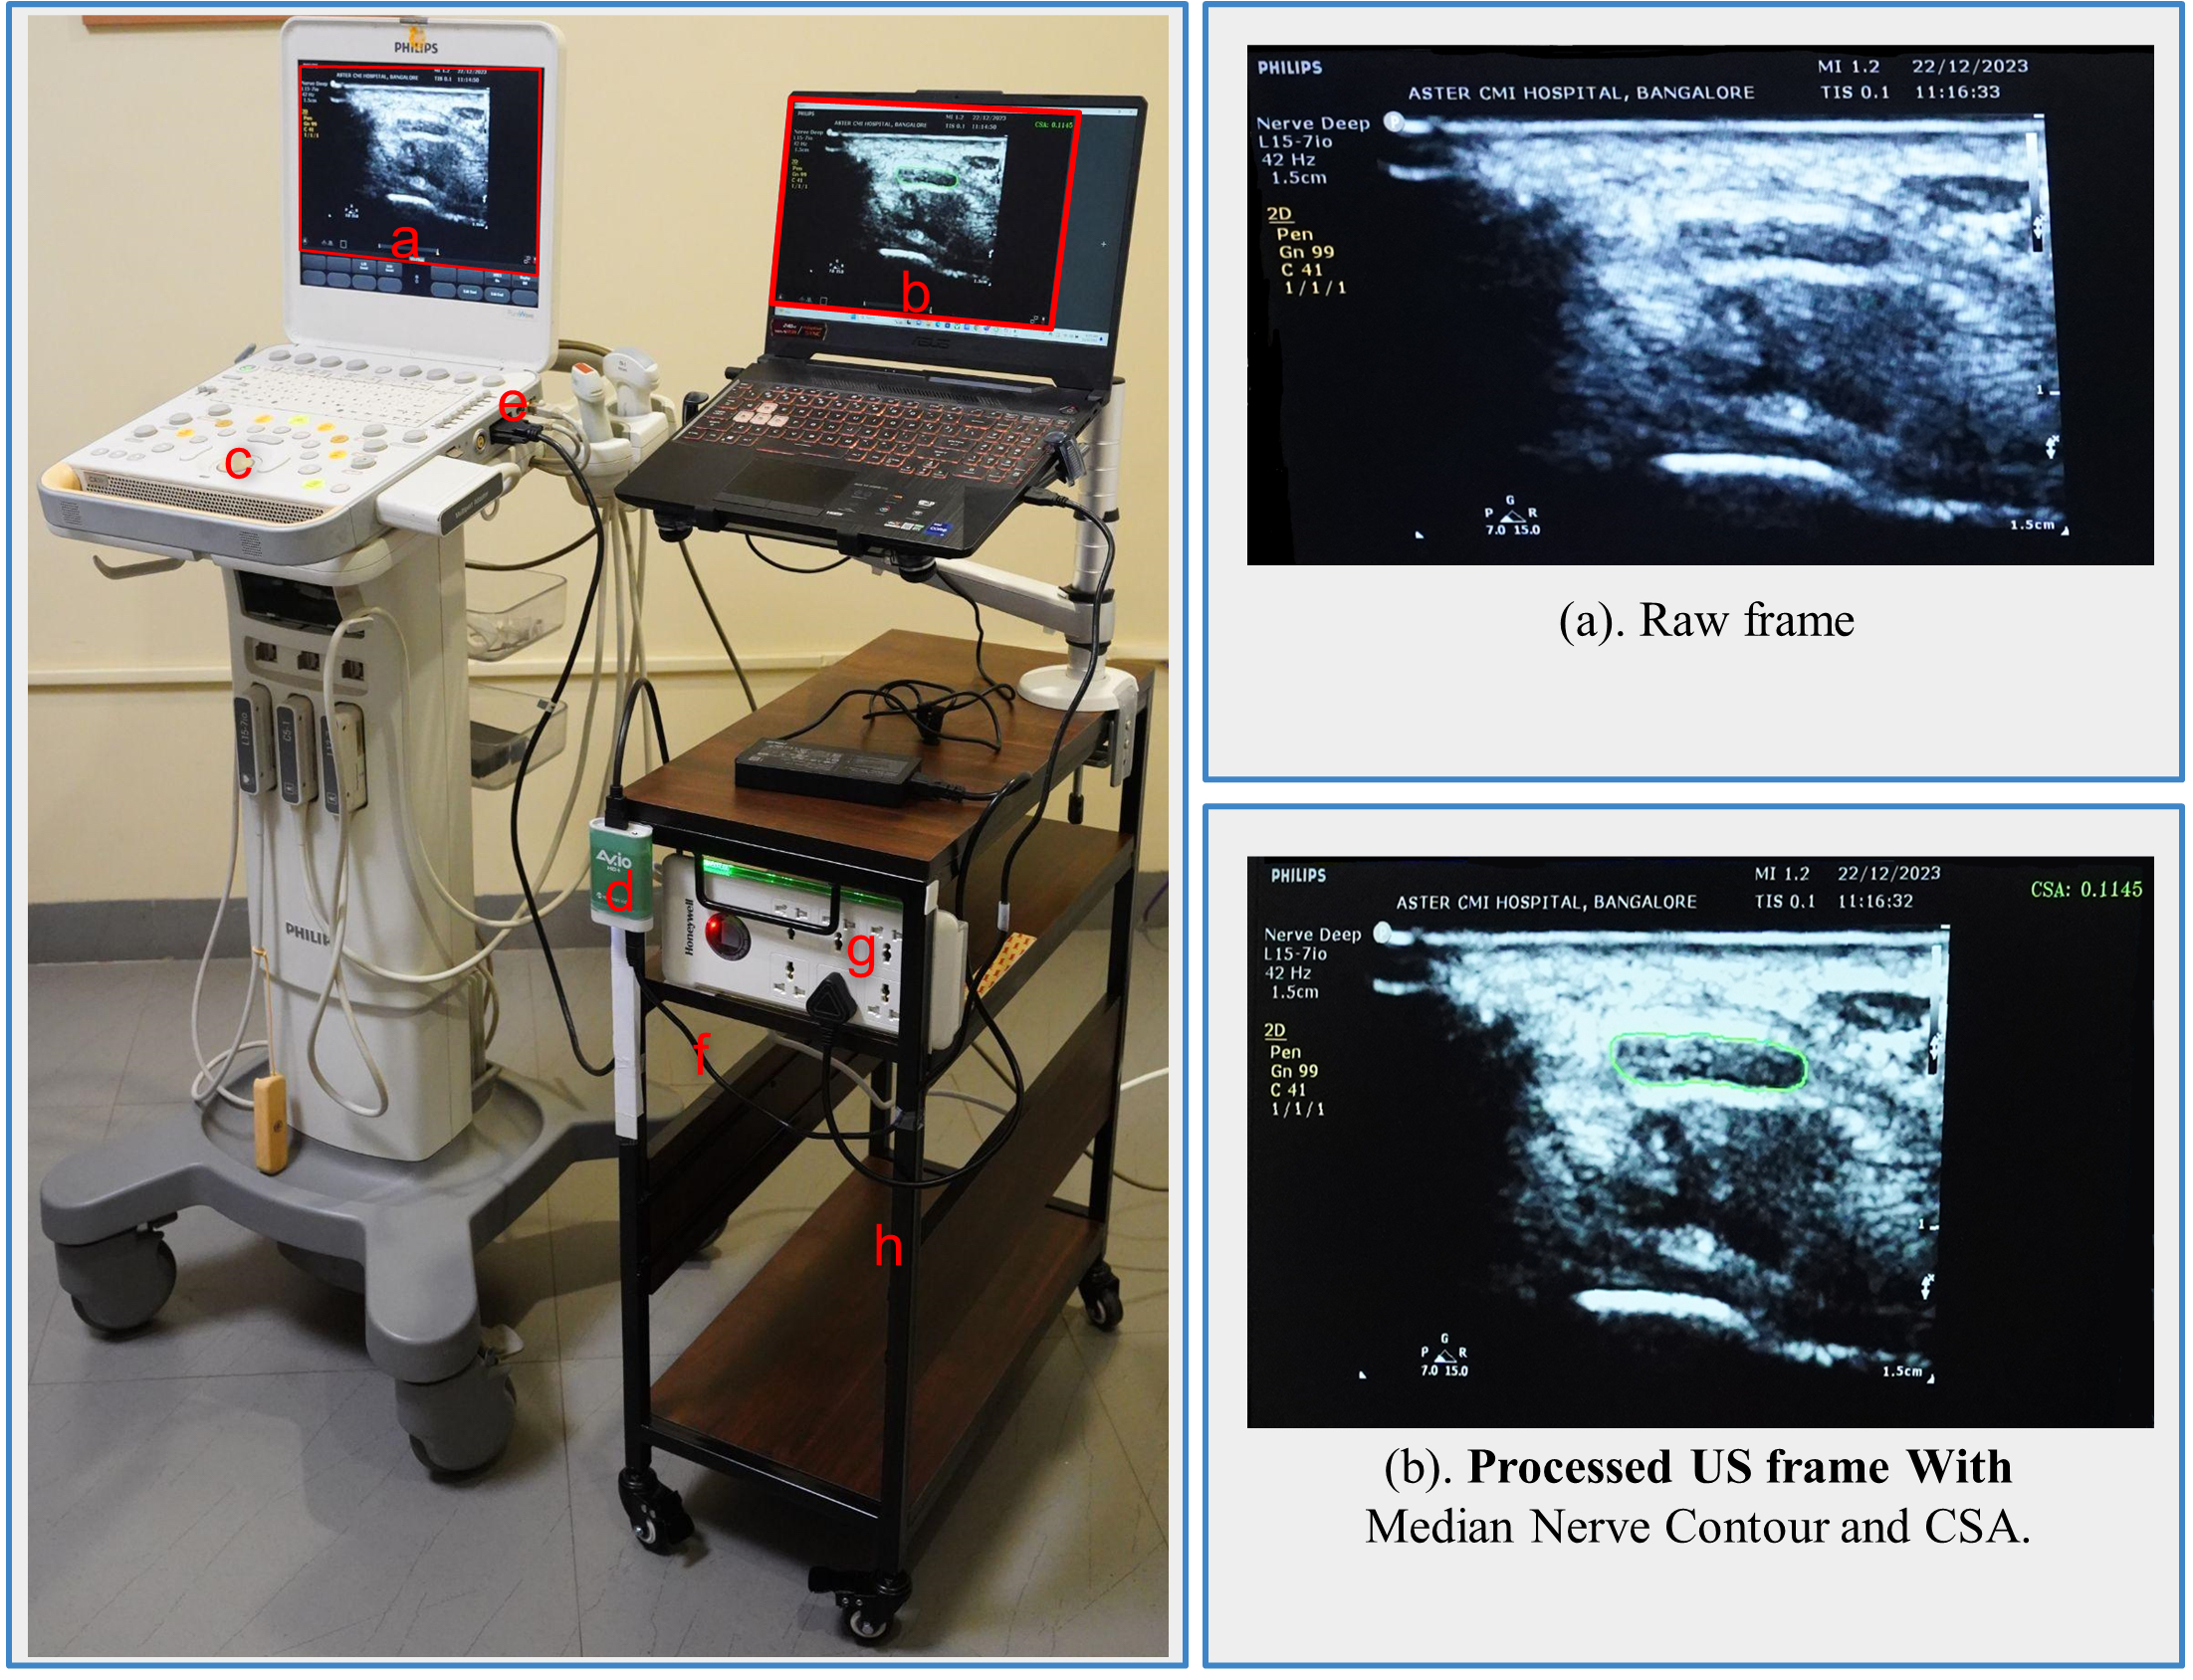
\includegraphics[width=\linewidth]{Figure1}}
    \caption{The physical system setup for Real-Time Median Nerve Segmentation includes the following main parts: (c). Philips cx50 ultrasound (US) machine(Input source) (d). Av.io Frame Grabber (e). DVI-to-HDMI interface (f).USB-B-to-USB-A interface (g). Switch box (power supply) (h). Portable wheeled table for the movable setup. The frame grabber was connected to the DVI output of the US machine. It is then connected via USB-B to a laptop, which serves as the computational device for executing the deep learning model.}
      \label{fig:clinical_setup}
\end{figure}

High-frequency alternating currents\cite{avendano2018peripheral,hopkins2007ultrasound} are used in peripheral nerve block therapy, requiring precise determination of the nerve diameter or cross-sectional area (CSA) to establish the minimum frequency for effective nerve block induction. Segmentation is crucial for diagnosing conditions such as CTS, guiding ultrasound-guided regional anesthesia (UGRA)\cite{marhofer2005ultrasound}, identifying nerve entrapment syndromes, and understanding nerve anatomy. Accurate segmentation of the median nerve in medical imaging enhances patient care by enabling precise surgical interventions. Regional anesthesia serves as an effective alternative to general anesthesia in many surgeries. Traditionally, needle guidance to target nerves has been conducted blindly, risking nerve injury and local anesthetic toxicity. The UGRA allows real-time visualization of nerves and needle placement, thereby reducing these risks. Precise segmentation of the median nerve improves patient outcomes, and the safety and effectiveness of surgical procedures. Existing clinical methods often lack metrics for identifying CTS, and procedures such as nerve conduction studies may cause patient discomfort.

Numerous tools have been developed to aid radiologists in segmenting the median nerve in ultrasound (US) images. Hadjerci et al. \cite{hadjerci2015ultrasound} proposed an automated method for median nerve localization for UGRA, employing a machine learning framework that includes despeckling filtering, feature extraction, and selection, followed by pixel-wise classification using a support vector machine with a Gaussian kernel. Similarly, \cite{hadjerci2016computer} introduced a computer-aided machine learning algorithm for median nerve localization. However, these techniques rely on manual feature extraction and selection, and the accuracy of the segmented images depends on the selected features.

In recent years, deep learning techniques have emerged as promising tools for medical ultrasound analysis, particularly for nerve segmentation. One study introduced a convolutional neural network (CNN) with spatiotemporal consistency for nerve segmentation \cite{hafiane2017deep}, whereas another study used similarity measures to track the median nerve during wrist motion \cite{wang2020mnt}. Huang et. al.\cite{huang2022attention} utilized the Attention-VGG16-UNet for median nerve segmentation at the wrist and trained the model using data from the wrist inlet. Automated frameworks, such as a U-Net-based model \cite{festen2021automated} and DeepNerve, which integrates MaskTrack with convolutional long short-term memory (LSTM) \cite{horng2020deepnerve}, have also been proposed. Comparative analyses evaluated the performance of pre-trained CNN models for median nerve localization/segmentation \cite{wu2021automated}, and a Mask R-CNN approach with additional layers to predict CSA \cite{di2022deep}.  A robot-assisted ultrasound imaging system was developed to enhance the monitoring of percutaneous needle insertion \cite{needleims}, autonomously restoring visibility when misalignment occurs, and achieving precise segmentation of the needle with minimal positional and angular errors in ex vivo porcine samples. Yeh et al. \cite{yeh2023real} introduced a simple, real-time instance segmentation model for the median nerve at the wrist, achieving state-of-the-art speed and accuracy, making it highly suitable for diagnosing CTS with dynamic ultrasonography. Wang et al. \cite{wangtnnls} recently proposed a lightweight encoder-decoder network called GREnet for generalized 2D medical image segmentation, including ultrasound images, that was prohibitively expensive for deployment in real-time. EU2-Net \cite{sarkarims} is a novel ensemble model that enhances the U2-Net architecture for breast ultrasound image segmentation by replacing conventional convolutional layers with separable convolutions, incorporating a weighted averaging ensemble mechanism with learnable weights, and utilizing an attention-aided triple feature fusion technique to improve segmentation accuracy, achieving state-of-the-art results on publicly accessible datasets. Recent work by Pan et. al \cite{pan2022} a novel two-stage method combining a cascaded segmentation network and a knowledge-based classification network to accurately recognize medullary thyroid carcinoma (MTC) from ultrasound images, achieving higher accuracy than experienced clinicians. Another recent study \cite{stenosismedphys} introduced VLSC-Net, a deep neural network-based approach for the precise segmentation and classification of dialysis access (DA) stenosis in ultrasound images, notably enhancing diagnostic accuracy and efficiency. Gujarati et al. \cite{gujarati2023transformer} used a modified vision transformer (VisTR) model to segment the median nerve from wrist to elbow, achieving superior segmentation accuracy. However, the model's high computational complexity and requirement for video input, which necessitates numerous frames and extensive spatial information, make it less practical for real-time clinical use.

Most methods have focused on segmenting the median nerve at the wrist, where localization is easier, and simple UNet-based architectures perform well. However, their performance declines from the wrist to the elbow because of the increased depth and rapid shape changes of the median nerve. UNet models struggle to capture long-range dependencies and complex spatial relationships, which are problematic in ultrasound image segmentation with rapidly changing foreground and background. In addition, many UNet-based methods lack effective metrics for identifying CTS, thereby limiting their clinical utility. Recent methods by Yeh et al. \cite{yeh2023real} focused on real-time instance segmentation using ultrasound for clinical use but were limited to the wrist region (not tested as a practical clinical application). Conversely, Gujarati et al. \cite{gujarati2023transformer} aimed to enhance the segmentation accuracy; however, this was less practical for real-time clinical use with ultrasound.

This study introduces a novel encoder-decoder-based architecture with a unique design that captures richer contextual information through a larger receptive field. It also incorporates a specialized network block to leverage the multiscale features and enhance the feature representation. These architectural changes resulted in a simple yet efficient deep learning model that addressed the current limitations. The goal was to develop an end-to-end, deep learning-based automated tool to aid sonographers in segmenting the median nerve at the wrist, mid-forearm, and elbow using ultrasound images. This study proposes \textcolor{red}{MNSeg-Net}, a lightweight, real-time, inference-supported, and efficient CNN model for median nerve segmentation from the wrist to the elbow using a single ultrasound video frame.



To evaluate the effectiveness of the proposed MNSeg-Net, several well-known deep learning models for medical image segmentation were selected as benchmarks. UNet~\cite{ronneberger2015u} and its variants (SegNet~\cite{badrinarayanan2017segnet}, ResUNet~\cite{diakogiannis2020resunet}, Attention-UNet~\cite{oktay2018attention}, UNet++~\cite{zhou2018unet++}, BASNet~\cite{qin2019basnet}, and U2Net~\cite{qin2020u2}) were included because they represent baseline encoder-decoder architectures with different enhancements, such as skip connections, attention mechanisms, and residual learning. BASNet and U2Net were selected because of their success in fine-grained object segmentation and hierarchical design, which aligns well with the requirements for median nerve localization in ultrasound. These benchmark models provide a comprehensive basis for evaluating the performance, computational efficiency, and clinical applicability of MNSeg-Net.


\textcolor{red}{The specific contributions of this study, encompassing architectural innovation, statistical validation, and clinical integration, are as follows:}

\begin{itemize}

\item \textcolor{red}{\textbf{Proposed MNSeg-Net Architecture:} Development of MNSeg-Net, a novel lightweight deep learning architecture designed for fully automated, real-time median nerve segmentation. The model integrates a computationally efficient redesigned U2Net backbone with a multi-scale feature fusion sub-network to effectively capture contextual information and enhance feature representation without adding the high computational overhead.}


\item \textcolor{red}{\textbf{Comprehensive and Statistically Rigorous Evaluation:} A rigorous evaluation of the proposed model against state-of-the-art segmentation networks. This study establishes the effectiveness of lightweight architectures through extensive statistical analysis and demonstrated that high segmentation accuracy and cross-sectional area (CSA) estimation can be achieved with significantly reduced parameter counts.}

\item \textcolor{red}{\textbf{Clinical Translation through Real-Time Integration:} Development and deployment of an end-to-end clinical workflow that integrates the deep learning model with real-time ultrasound data. This contribution includes a custom graphical interface for real-time visualization and automatic CSA computation, validated on a diverse dataset of healthy subjects and patients with carpal tunnel syndrome (CTS) to assess clinical feasibility.}



\end{itemize}







\section{Methods}

\subsection{Data Acquisition and Preparation}
This study used two distinct datasets: Dataset-1 for experimental evaluation and Dataset-2 for clinical validation.

\subsubsection{Dataset-1: Experimental Dataset}  
The primary dataset (Dataset-1) was sourced from the Aster-CMI Hospital, Bangalore, India, and acquired using a Philips CX50 ultrasound machine equipped with a Philips L15-7io hockey-stick transducer probe (frequency range: 7–15 MHz). The participants were positioned facing the examiner with their forearms and fingers extended, as shown in Fig. ~\ref{fig:real_time_screen_shots}. Imaging was performed at a depth of 3 cm, and each subject’s scan was recorded as an 8-second video (approximately 312 frames at 39 fps), with each frame measuring $800 \times 600$ pixels. The dataset included 100 subjects, annotated by an expert sonographer. For each video, the first 300 frames were used for labeling, resulting in 30,000 annotated frames. Annotations were generated using ImageJ~\cite{ferreira2012imagej}, a free NIH image analysis tool, and stored as binary segmentation masks for the median nerve. The 100-subject dataset was split into training, validation, and test sets with 80, 10, and 10 subjects, respectively. Data augmentation via horizontal flipping was applied to the training set, increasing the total to 48,000 images. The validation and test sets each comprised 3,000 images (300 frames per subject $\times$ 10 subjects).


\subsubsection{Dataset-2: Clinical Evaluation Dataset}  
To assess clinical applicability, a separate dataset (Dataset-2) comprising 30 subjects was collected for real-time evaluation. This dataset included both NORMAL and CTS-positive cases, with 18 subjects categorized as NORMAL and 12 as CTS-positive based on clinical criteria, including a CSA threshold of 12 mm\textsuperscript{2} \cite{ghasemi2017determination,nkrumah2020ultrasonography,falsetti2022novel}. Each subject contributed a video recorded under the same imaging setup as Dataset-1, with six clinician annotations per subject, focused at the wrist level. These annotations were used to compare the MNSeg-Net-predicted CSA (CSA\textsubscript{Cal}) with the clinician-annotated CSA (CSA\textsubscript{Act}) for statistical and clinical reliability analyses.

All Ethical and experimental procedures were approved by the Internal Ethical Committee of the Aster-CMI Hospital, Bangalore, India (Approval No. Aster/IEC/049/2020-21, dated June 27, 2020). Written informed consent was obtained from all participants. The study population had a male-to-female ratio of 1:3, with participants aged between 35 and 65 years. Individuals with prior major nerve surgery were excluded because of the possibility of postoperative anatomical alterations.





\subsection{Proposed Median Nerve Segmentation Network}
\noindent
The proposed Median Nerve Segmentation Network, referred to as MNSeg-Net, is a lightweight architecture designed for accurate, real-time segmentation of the median nerve in ultrasound images. While inspired by the U2Net framework \cite{qin2020u2}, MNSeg-Net introduces several important modifications to reduce computational cost and enable deployment on resource-constrained clinical hardware, without sacrificing segmentation performance.

The overall architecture of MNSeg-Net is organized into two components: (i) a Main-Network, which is a lightweight redesign of U2Net optimized for real-time inference, and (ii) a Sub-Network, a multi-scale feature fusion (MSFF) module that efficiently aggregates encoder features to enhance contextual representation. An overview of the complete architecture, including the main encoder–decoder backbone and the MSFF sub-network, is shown in Fig.~\ref{fig:MNSeg_Net_architecture}, while the detailed UNet block configurations are provided in Fig.~1 of the supplementary materials.




\subsubsection{Main-Network: Lightweight Redesign of the U2Net}
\noindent
The original U2Net~\cite{qin2020u2} employs a fully nested U-structure with exponentially varying filter counts, resulting in a model of approximately 44M parameters that is computationally expensive for real-time or edge deployment. In contrast, the proposed main network adopts a lightweight redesign in which the encoder (E1–E5) and bottleneck (E6) are mirrored by the decoder (D1–D5), with each stage implemented as a compact residual UNet block using uniform filter allocation (64 filters in outer blocks and 32 in inner blocks). Each block includes a single residual connection to enhance the gradient flow while reducing redundancy. This modification reduces the parameter count to 2.46M and lowers the FLOPs by more than an order of magnitude, enabling real-time inference without sacrificing the representational capability. To further balance accuracy and efficiency, deeper residual U-blocks are used in the early encoder–decoder stages (E1–E3 and D1–D3), whereas the later stages (E4–E5 and D4–D5) adopt shallower blocks to reduce computation. Additionally, dilated convolutions replace pooling and upsampling in the deeper encoder (E5), bottleneck (E6), and final decoder (D5), thereby enlarging the receptive field while preserving the fine spatial details crucial for nerve boundary localization. Together, these modifications provide a compact yet powerful backbone that retains the contextual strengths of U2Net while being optimized for clinical applications requiring efficient and accurate real-time segmentation.

\begin{figure*} [htbp]
\centering
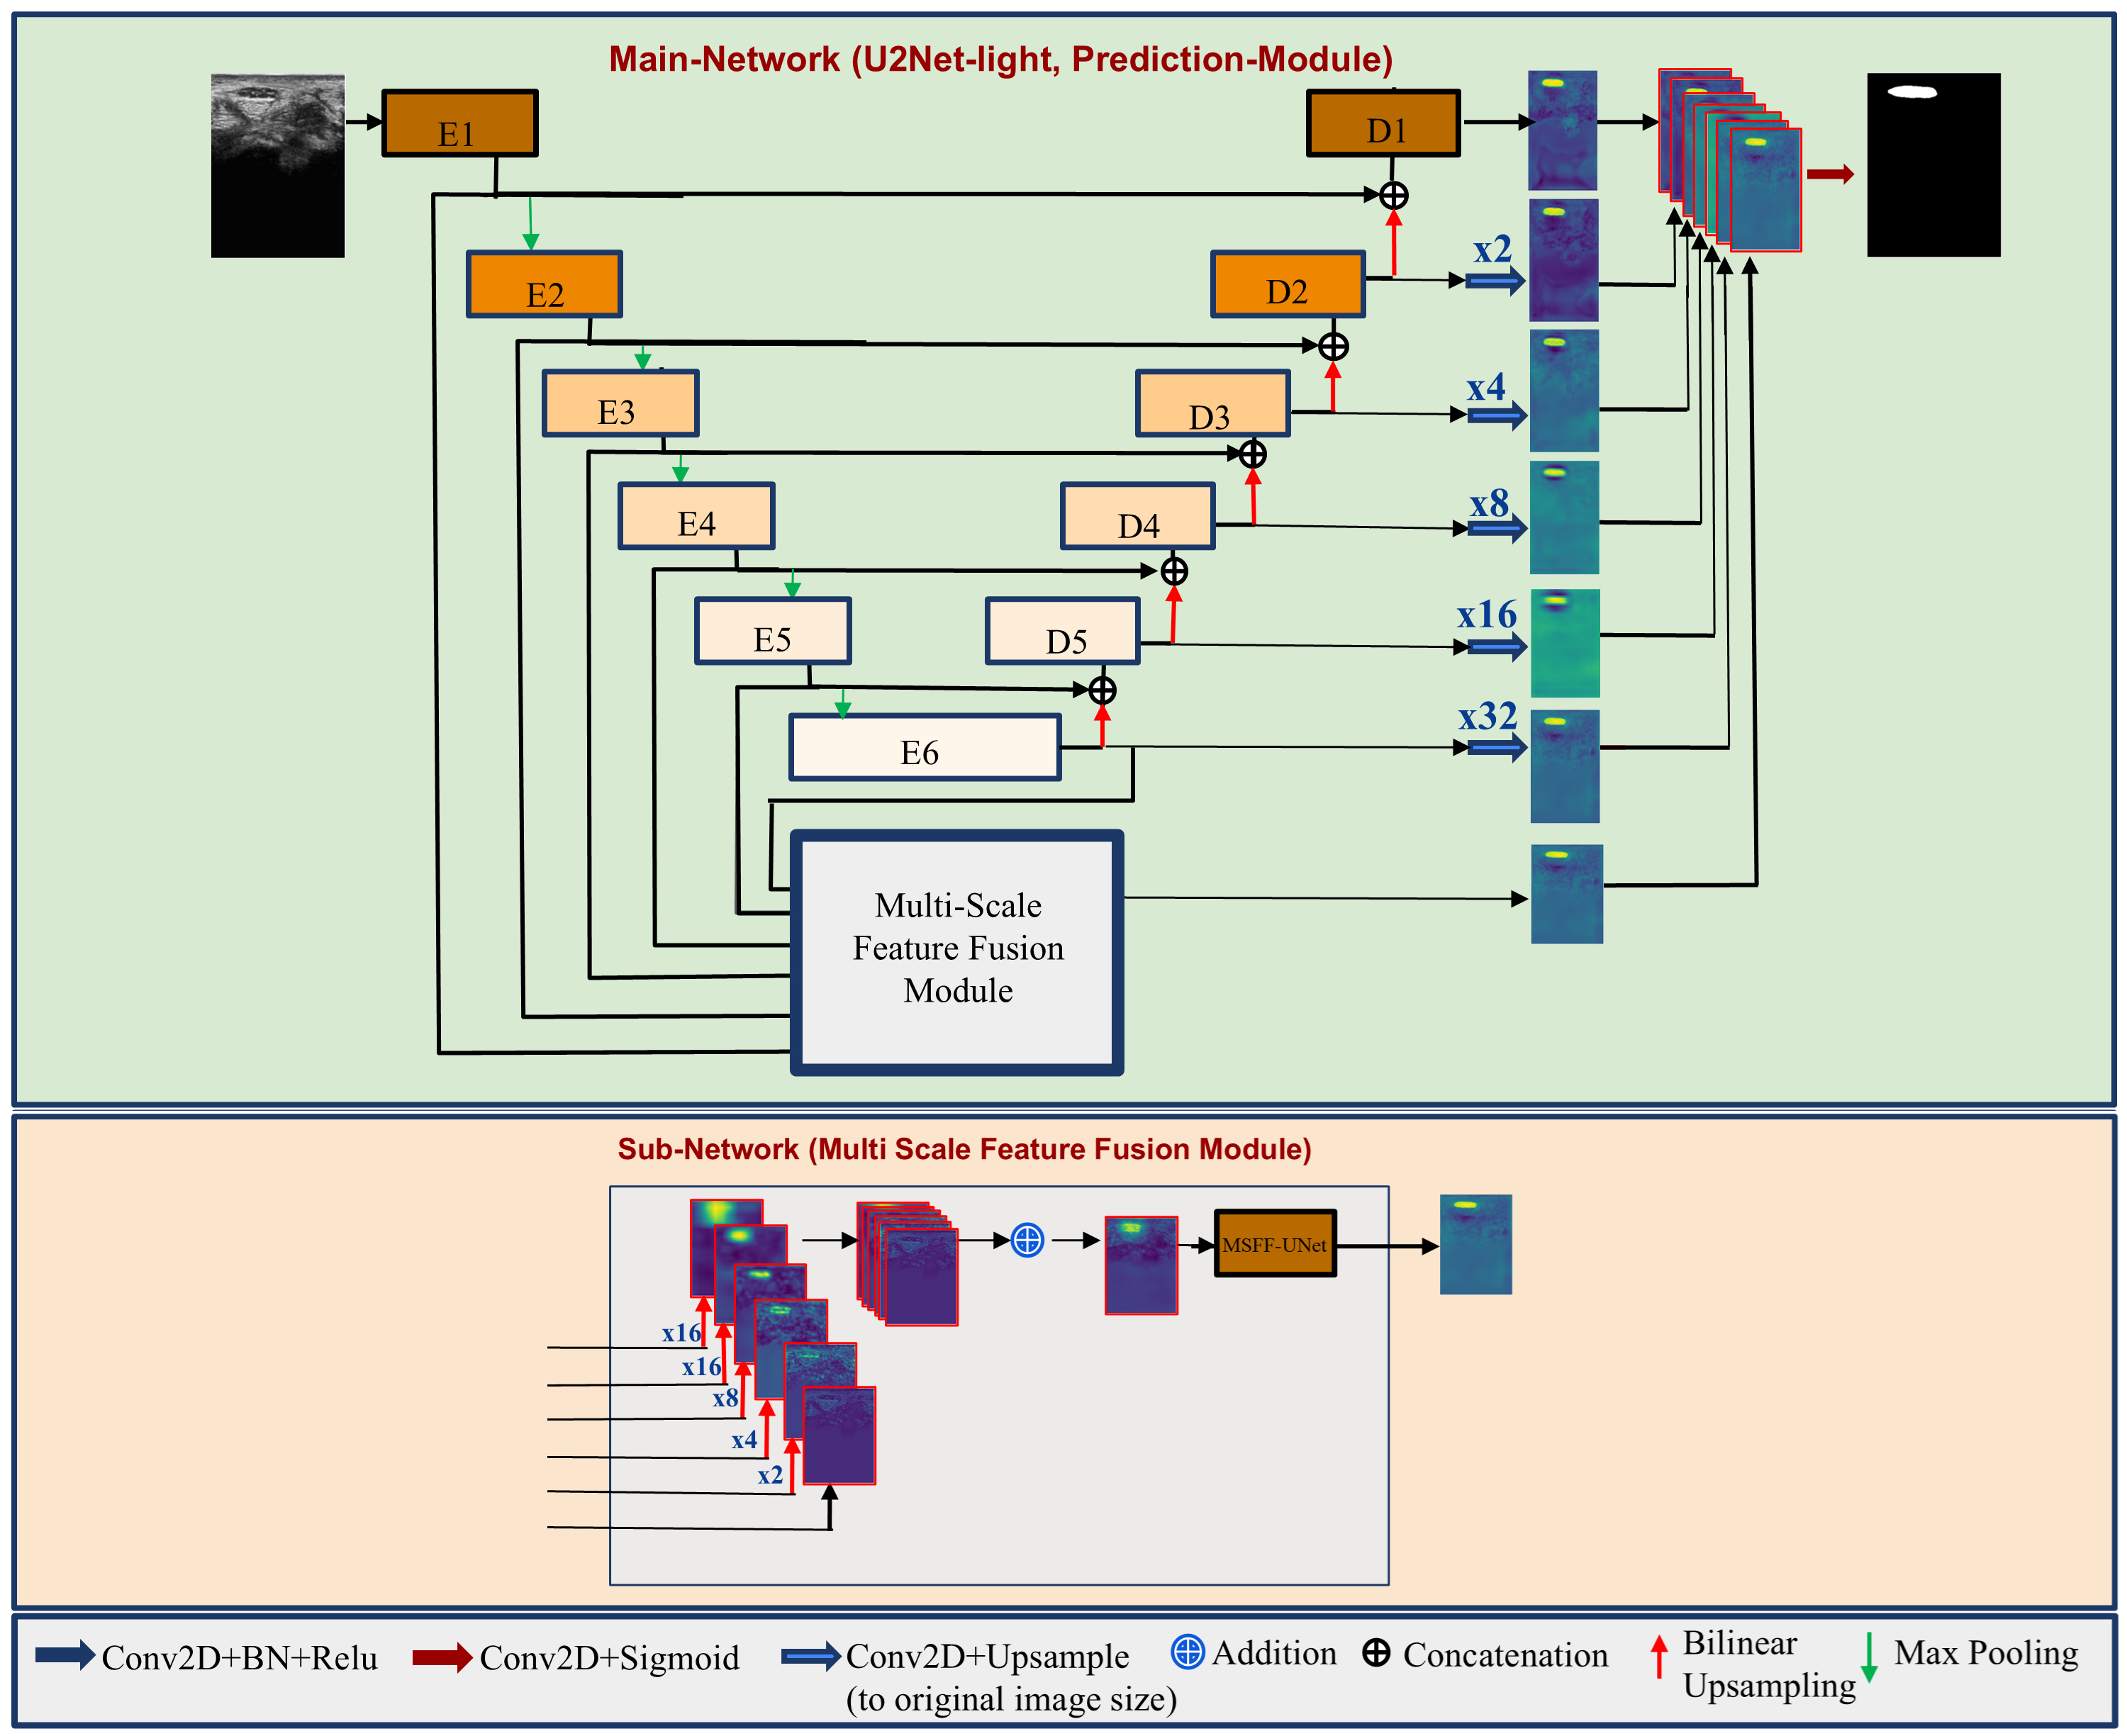
\includegraphics[width=\linewidth]{Figure2}
\caption{The proposed MNSeg-Net architecture for Median Nerve Segmentation with deep supervision and sub-network module for multi-scale feature fusion. (a) Main-network as prediction module, (b) Sub-network for multi-scale feature fusion. {Detailed UNet block configurations used in MNSeg-Net were provided in Fig. 1 of supplementary information.}}
  \label{fig:MNSeg_Net_architecture}
\end{figure*}



\begin{figure*}[htbp]
    \centering
    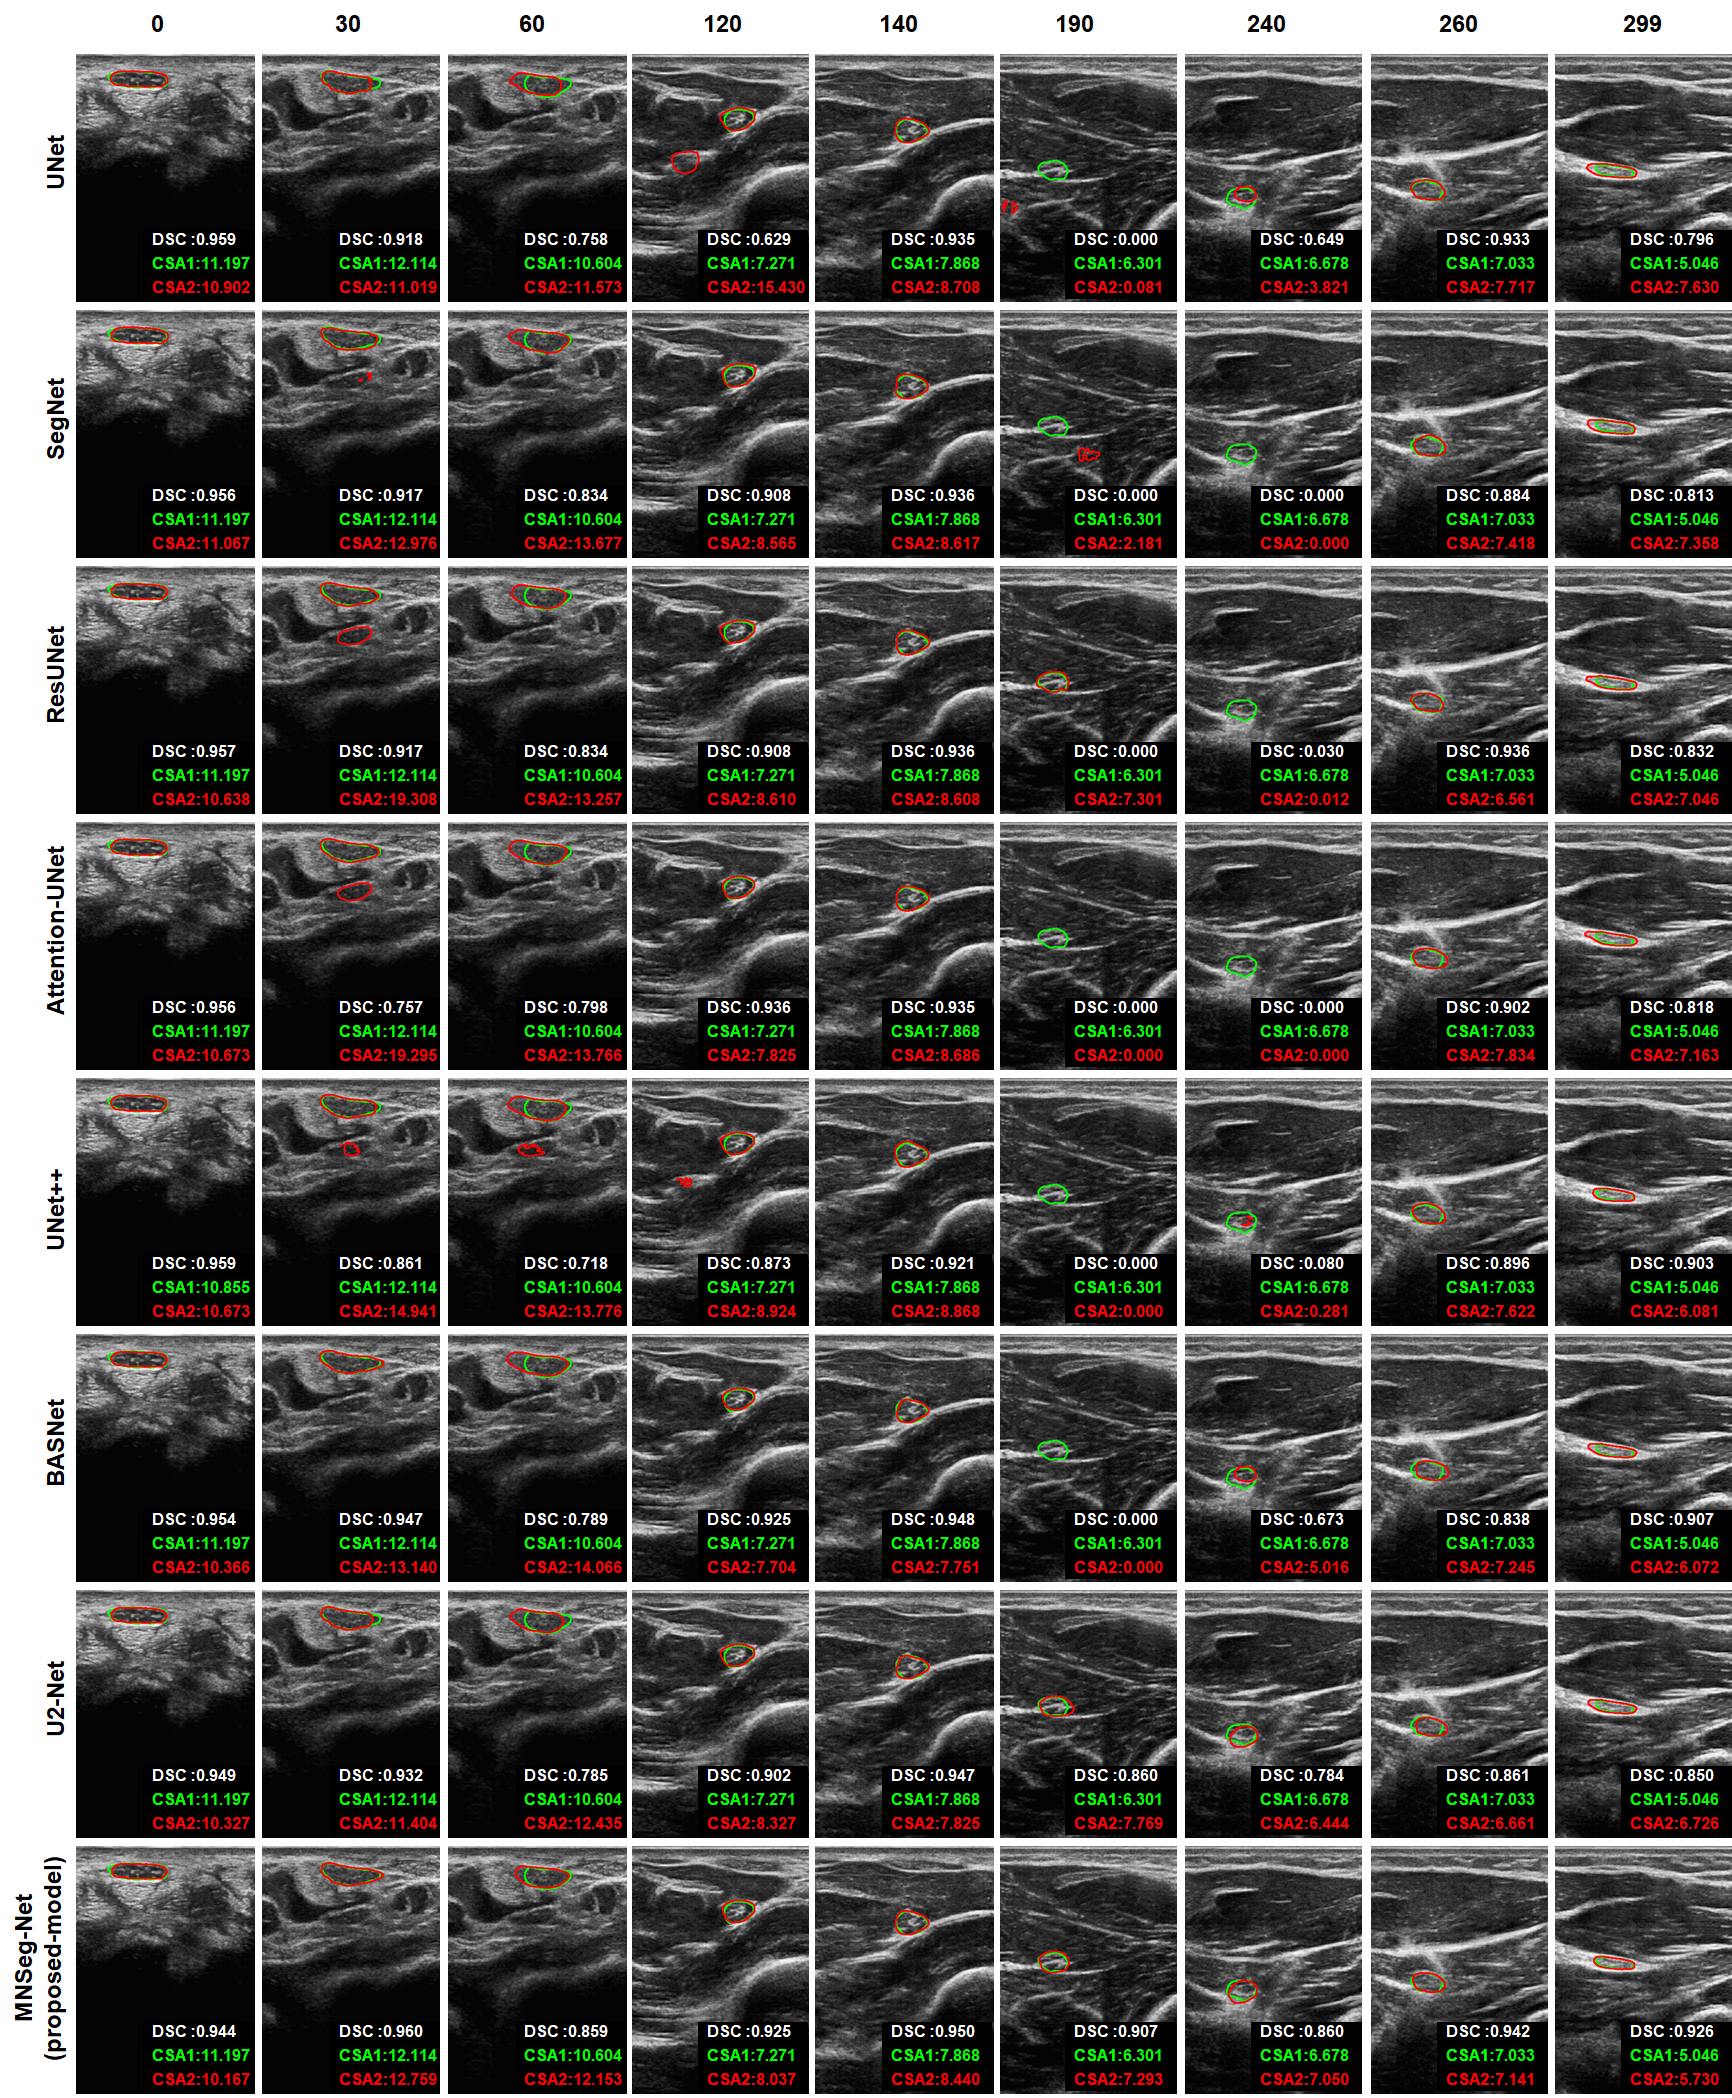
\includegraphics[width=0.99\textwidth]{Figure3}
    \caption{Example segmentation of the median nerve using the methods discussed in this work for subject-1. The green contour indicates expert annotation, and the red contour indicates the result obtained for the corresponding method, as indicated in each row. The associated frame number is given at the top of every image (0 corresponds to the start of the wrist region, and 299 corresponds to the elbow region), and the bottom of each frame has the corresponding computed cross-sectional area (CSA) from the expert and model in green and red, respectively.
}
    \label{fig:sample_segmented_images_of_patient_1}
\end{figure*}

\subsubsection{Sub-network: Multi-Scale Feature Fusion}
\noindent
In addition to the main encoder–decoder backbone, MNSeg-Net incorporates a dedicated sub-network module for MSFF, designed to enhance segmentation performance by leveraging complementary features across encoder stages. Specifically, feature maps from all encoder blocks (E1–E5) and the bottleneck (E6) are extracted, resized to the input image resolution, and concatenated to form a multiscale representation that captures both local fine-grained details and global contextual information. This fused representation is then processed by a lightweight UNet, which transforms the multichannel input into a compact single-channel feature map at full resolution. By reusing encoder features rather than introducing new feature extraction layers, the MSFF module introduces a minimal additional computational cost while significantly improving the ability to localize nerve boundaries. Finally, the output of this sub-network is integrated with the decoder outputs (D1–D5) and bottleneck (E6) during the final prediction stage, ensuring that both multi-scale context and deep supervised features contribute to the final segmentation mask.

Overall, the MSFF sub-network serves as a compact yet powerful enhancement to the main backbone. By reusing the multi-scale features from E1–E6 and fusing them through a lightweight UNet, the contextual representation is enriched while keeping the computation minimal. This design ensures that MNSeg-Net effectively captures both fine local details and global structures, making the segmentation output more accurate and reliable without sacrificing efficiency.




%\vspace{-2pt}
\begin{table}[ht]
\centering
\caption{Comparison between the proposed MNSeg-Net and the full-size U2Net model.}

\scalebox{0.5}{
\begin{tabular}{llcccclccccl}
\hline
&
& \multicolumn{5}{c}{\textbf{Proposed MNSeg-Net}} 
& \multicolumn{5}{c}{\textbf{U2Net (Full size)}} \\
\hline

\textbf{Type}
&\textbf{Block}
& \textbf{\shortstack{RAM\\Occupied\\(MB)}} 
& \textbf{\shortstack{Module\\Size\\(MB)}} 
& \textbf{\shortstack{Comput.\\(G. FLOPS)}} 
& \textbf{\shortstack{Params \\(M)}} 
& \textbf{\shortstack{Output \\(SHAPE)}} 
& \textbf{\shortstack{RAM\\Occupied\\(MB)}} 
& \textbf{\shortstack{Module\\Size\\(MB)}} 
& \textbf{\shortstack{Comput.\\(G. FLOPS)}} 
& \textbf{\shortstack{Params \\(M)}} 
& \textbf{\shortstack{Output \\(SHAPE)}} \\

\hline

\multirow{5}{*}{\textbf{\shortstack{Encoder\\Blocks}}}        

 & E1 & 807.46 & 0.79 & 9.6 & 0.206&64x448x320 & 807.46 & 0.79 & 9.600 & 0.206 &64x448x320\\ 
& E2 & 210.85 & 0.81 & 3.65 & 0.213&64x224x160 & 351.20 & 1.17 & 6.981 & 0.306 &128x448x320\\ 
& E3 & 53.24 & 0.71 & 0.914 & 0.185&64x112x80 & 179.30 & 4.23 & 6.958 & 1.109 &256x112x80\\ 
& E4 & 13.76 & 0.60 & 0.228 & 0.158&64x56x40 & 102.84 & 15.21 & 6.947 & 3.987 &512x56x40\\
& E5 & 6.21 & 0.60 & 0.089 & 0.158&64x28x20 & 38.28 & 38.28 & 5.620 & 10.035 &512x28x20\\ \hline
\textbf{Bottle Neck} & E6 & 2.00 & 0.60 & 0.022 & 0.158&64x14x10 & 49.49 & 38.28 & 1.405 & 10.035&512x14x10 \\ \hline
\multirow{5}{*}{\textbf{\shortstack{Decoder\\Blocks}}}        
& D5 & 6.48 & 0.74 & 0.109 & 0.194&64x28x20 & 93.22 & 47.28 & 6.942 & 12.394 &512x28x20\\ 
& D4 & 14.45 & 0.74 & 0.311 & 0.194&64x56x40 & 75.53 & 16.33 & 7.603 & 4.280 &256x56x40\\ 
& D3 & 55.57 & 0.85 & 1.245 & 0.222&64x112x80 & 122.70 & 4.51 & 7.610 & 1.182 &128x112x80\\ 
& D2 & 219.74 & 0.95 & 4.98 & 0.250&64x224x160 & 237.52 & 1.24 & 7.623 & 0.324 &64x224x160\\ 
& D1 & 876.09 & 1.06 & 19.922 & 0.278&64x448x320 & 753.05 & 0.53 & 14.952 & 0.139&64x224x160 \\ \hline

\textbf{MSFF-module} & MSFF-UNet & 877.05 & 0.92 & 14.646 & 0.241&64x448x320 & - & - & - & -&-\\ \hline
\textbf{Conv (projection) + Concat} & &-&-&-&-&7x448x320 &-&-&-&-&6x448x320\\ \hline

\textbf{Out Conv} &Out Conv &-&-&-&-&1x448x320 &-&-&-&-&1x448x320\\ \hline

\textbf{Overall} & - & 3142.8 & 9.37 & 55.716 & 2.458&1x448x320 & 2810.59 & 167.85 & 82.243 & 43.996 &1x448x320\\ \hline
\end{tabular}}
\label{tab:mnsnet_u2net_comparison}
\end{table}
%\vspace{-15pt}

\subsubsection{MNSeg-Net Architectural Contributions}
\noindent
The proposed MNSeg-Net integrates a lightweight adaptation of U2Net as the main network together with a novel MSFF module as a sub-network. Several architectural enhancements have been introduced to achieve this efficient design. Specifically, the encoder (E1–E5, E6) and decoder (D1–D5) blocks of the original U2Net were replaced with compact residual UNet (RSU) blocks, each featuring a single residual connection to improve the gradient flow while reducing the redundancy. Unlike the original U2Net, which employs an exponential variation in filter counts, the redesigned architecture adopts a uniform filter allocation (64 in the outer blocks and 32 in the inner blocks), thereby reducing the number of parameters and substantially lowering the computational complexity. Side-output layers were retained to support deep supervision and enhance the training stability. Furthermore, a novel MSFF module was introduced, employing a half-UNet-style decoder that directly upsamples and fuses multi-scale features from the encoder outputs (E1–E6), producing a compact and context-rich representation with minimal memory and computational overhead requirements. These combined architectural optimisations make MNSeg-Net considerably lighter than the original U2Net while maintaining competitive segmentation accuracy.

A detailed analytical derivation of the relationship between model parameters, computational complexity, memory consumption, and clinical deployability, including explicit parameter-scaling formulations for RSU blocks and the overall MNSeg-Net architecture, is provided in the section 1 of the Supplementary Material.

In addition to these technical contributions, the overall design of MNSeg-Net is purposefully aligned with clinical translation. By combining low computational demand with accurate segmentation, the model supports deployment in fully automated, real-time clinical setups for median nerve segmentation and CSA estimation.


Consequently, MNSeg-Net achieves real-time inference with only 2.46 million parameters and approximately 56 GFLOPs per image. A detailed comparison of the computational requirements between MNSeg-Net and the original U2Net is provided in Table~\ref{tab:mnsnet_u2net_comparison}, based on an input size of $448 \times 320$.



\begin{table}[h]
  \centering
  \caption{Deep learning models Specifications utilised in this work and their corresponding inference time}
  \label{tab:model_specs}
  \scalebox{0.73}{
  \begin{tabular}{lccccccc}
    \hline
    \textbf{Model} 
    & \textbf{\shortstack{Model \\Size\\(MB)}} 
    & \textbf{\shortstack{No. of\\Parameters\\(M)}} 
    & \textbf{\shortstack{Comput.\\(GFLOPs)}} 
    & \textbf{\shortstack{Inference\\Memory\\(MB)}} 
    & \textbf{\shortstack{Training\\Time\\(Min/Epoch)}} 
    & \textbf{\shortstack{Inference\\Speed\\(FPS)}} 
    & \textbf{\shortstack{Inference\\Time\\(ms/frame)}} \\
    \hline
    UNet~\cite{ronneberger2015u}             & 96.12  & 25.2   & 72.60   & 1854 & 20 & 71  & 14.08 \\
    SegNet~\cite{badrinarayanan2017segnet}   & 112.32 & 29.44  & 87.74   & 2781 & 30 & 66  & 15.15 \\
    ResUNet~\cite{diakogiannis2020resunet}   & 157.60 & 39.37  & 111.63  & 2472 & 40 & 38  & 26.32 \\
    Attention-UNet~\cite{oktay2018attention} & 152.20 & 38.01  & 166.00  & 3702 & 40 & 29  & 34.48 \\
    UNet++~\cite{zhou2018unet++}             & 146.60 & 36.62  & 302.43  & 4984 & 40 & 19  & 52.63 \\
    BASNet~\cite{qin2019basnet}             & 332.11 & 87.06  & 278.91  & 6103 & 40 & 20  & 50.00 \\
    U2Net~\cite{qin2020u2}                  & 167.88 & 44.01  & 82.53   & 2978 & 30 & 40  & 25.00 \\
    \textbf{\shortstack{MNSeg-Net\\(Proposed)} }          & \textbf{9.40}  & \textbf{2.46}  & \textbf{56.00}   & \textbf{3143} & \textbf{30} & \textbf{43} & \textbf{23.26} \\
    \hline
  \end{tabular}}
\end{table}


\section*{Training}\label{sec:training_section}
The proposed model was trained using a deep supervision strategy, in which losses were applied not only to the final network output but also to the intermediate outputs to enhance the gradient flow and stabilize the optimization. Specifically, eight outputs were considered: the final output, five decoder blocks, a bottleneck, and a subnetwork module. Each output was optimized using the same hybrid loss function, which combined three complementary components: SSIM loss, log-cosh loss, and binary cross-entropy (BCE) loss. loss. This hybrid formulation leverages the perceptual sensitivity of SSIM, the robustness of log-cosh to outliers, and the probabilistic classification strength of BCE, thereby ensuring both structural fidelity and pixel-level accuracy. The overall training loss was obtained by summing the hybrid loss values across all eight supervised outputs. Although this comprehensive deep supervision improves gradient propagation and supports robust learning, it also requires a relatively high GPU memory. Training converged within seven epochs, taking approximately 5.25 hours of computational time.




\subsection{Testing and CSA Computation}
\noindent
After completing end-to-end training, the architecture was used to classify each pixel of the test image into two categories: background and median nerve.  Each pixel was assigned a label based on the highest probability score among the two categories. In addition, the proposed method automatically computes the CSA of the median nerve by calibrating the dimensions of individual pixels. Specifically, for the $\text{3 cm}$ depth settings, each pixel occupied an area of $0.00432 mm^{2}$, and for the $1.5 cm$ depth settings, it was $0.00119 mm^{2}$. The CSA was computed by multiplying the single-pixel area by the number of median nerve pixels.
%\vspace{-10pt}
\subsection{Quantitative Performance Evaluation}
\noindent
The effectiveness of the proposed deep learning model was assessed using metrics such as the DSC\cite{zou2004statistical}, precision (Prec), recall(Rec), and the Hausdorff distance (HD)\cite{huttenlocher1993comparing}. The DSC evaluates the overlap between expert annotations and predicted segmentation masks, with higher values indicating better alignment. Precision measures the proportion of true-positive predictions among all positive predictions, whereas recall assesses the proportion of true-positive predictions among all actual positives. HD measures the furthest distance from any point in one set to the nearest point in the other set, offering a numerical assessment of segmentation accuracy. 

%\vspace{-15pt}
\subsection{Implementation}
All the deep learning models were trained using PyTorch and the Adam optimizer \cite{kingma2014adam}. The models were trained using various loss functions, including the dice loss \cite{sudre2017generalised}, (BCE) \cite{de2005tutorial}, logcosh loss \cite{jadon2020survey}, and a custom hybrid loss function that combines the logcosh loss, BCE loss, and SSIM loss \cite{wang2004image, qin2019basnet}. Computations, including model training, were performed on a Linux workstation with an Intel i9 9920X CPU, 128 GB RAM, and two NVIDIA Quadro RTX 8000 GPUs with 48 GB of memory each. The hybrid loss ($loss_{Hybrid}$) was selected after extensive experimentation for its superior performance, defined as
\begin{equation}
 loss_{Hybrid}=loss_{SSIM}+loss_{logcosh}+loss_{BCE}.
\end{equation}


During the training process, the models were trained at various learning rates, including \(1 \times 10^{-3}\), \(1 \times 10^{-4}\), \(5 \times 10^{-4}\), and \(5 \times 10^{-5}\). The UNet-based models exhibited stable training at \(1 \times 10^{-4}\). However, the training time required was relatively high for learning rates of \(1 \times 10^{-5}\) and \(5 \times 10^{-5}\). Similarly, the proposed MNSeg-Net model exhibited stable training at \(1 \times 10^{-4}\) and comparable results at \(5 \times 10^{-4}\), and the training time required was relatively high for a learning rate \(5 \times 10^{-5}\). Because all the models were encoder-decoder-based, the training process was stable. All models, including the proposed model, were trained from scratch, and the best model was chosen based on the minimum validation loss. For a fair comparison, all the UNet-based models were considered to have the same depth (in terms of the encoder and decoder blocks) and the same number of filters in each stage. The Adam optimizer was used to train all models. In all experiments, training was continued for 30 epochs to maintain consistency.


\begin{figure*}[htbp]
    \centering
    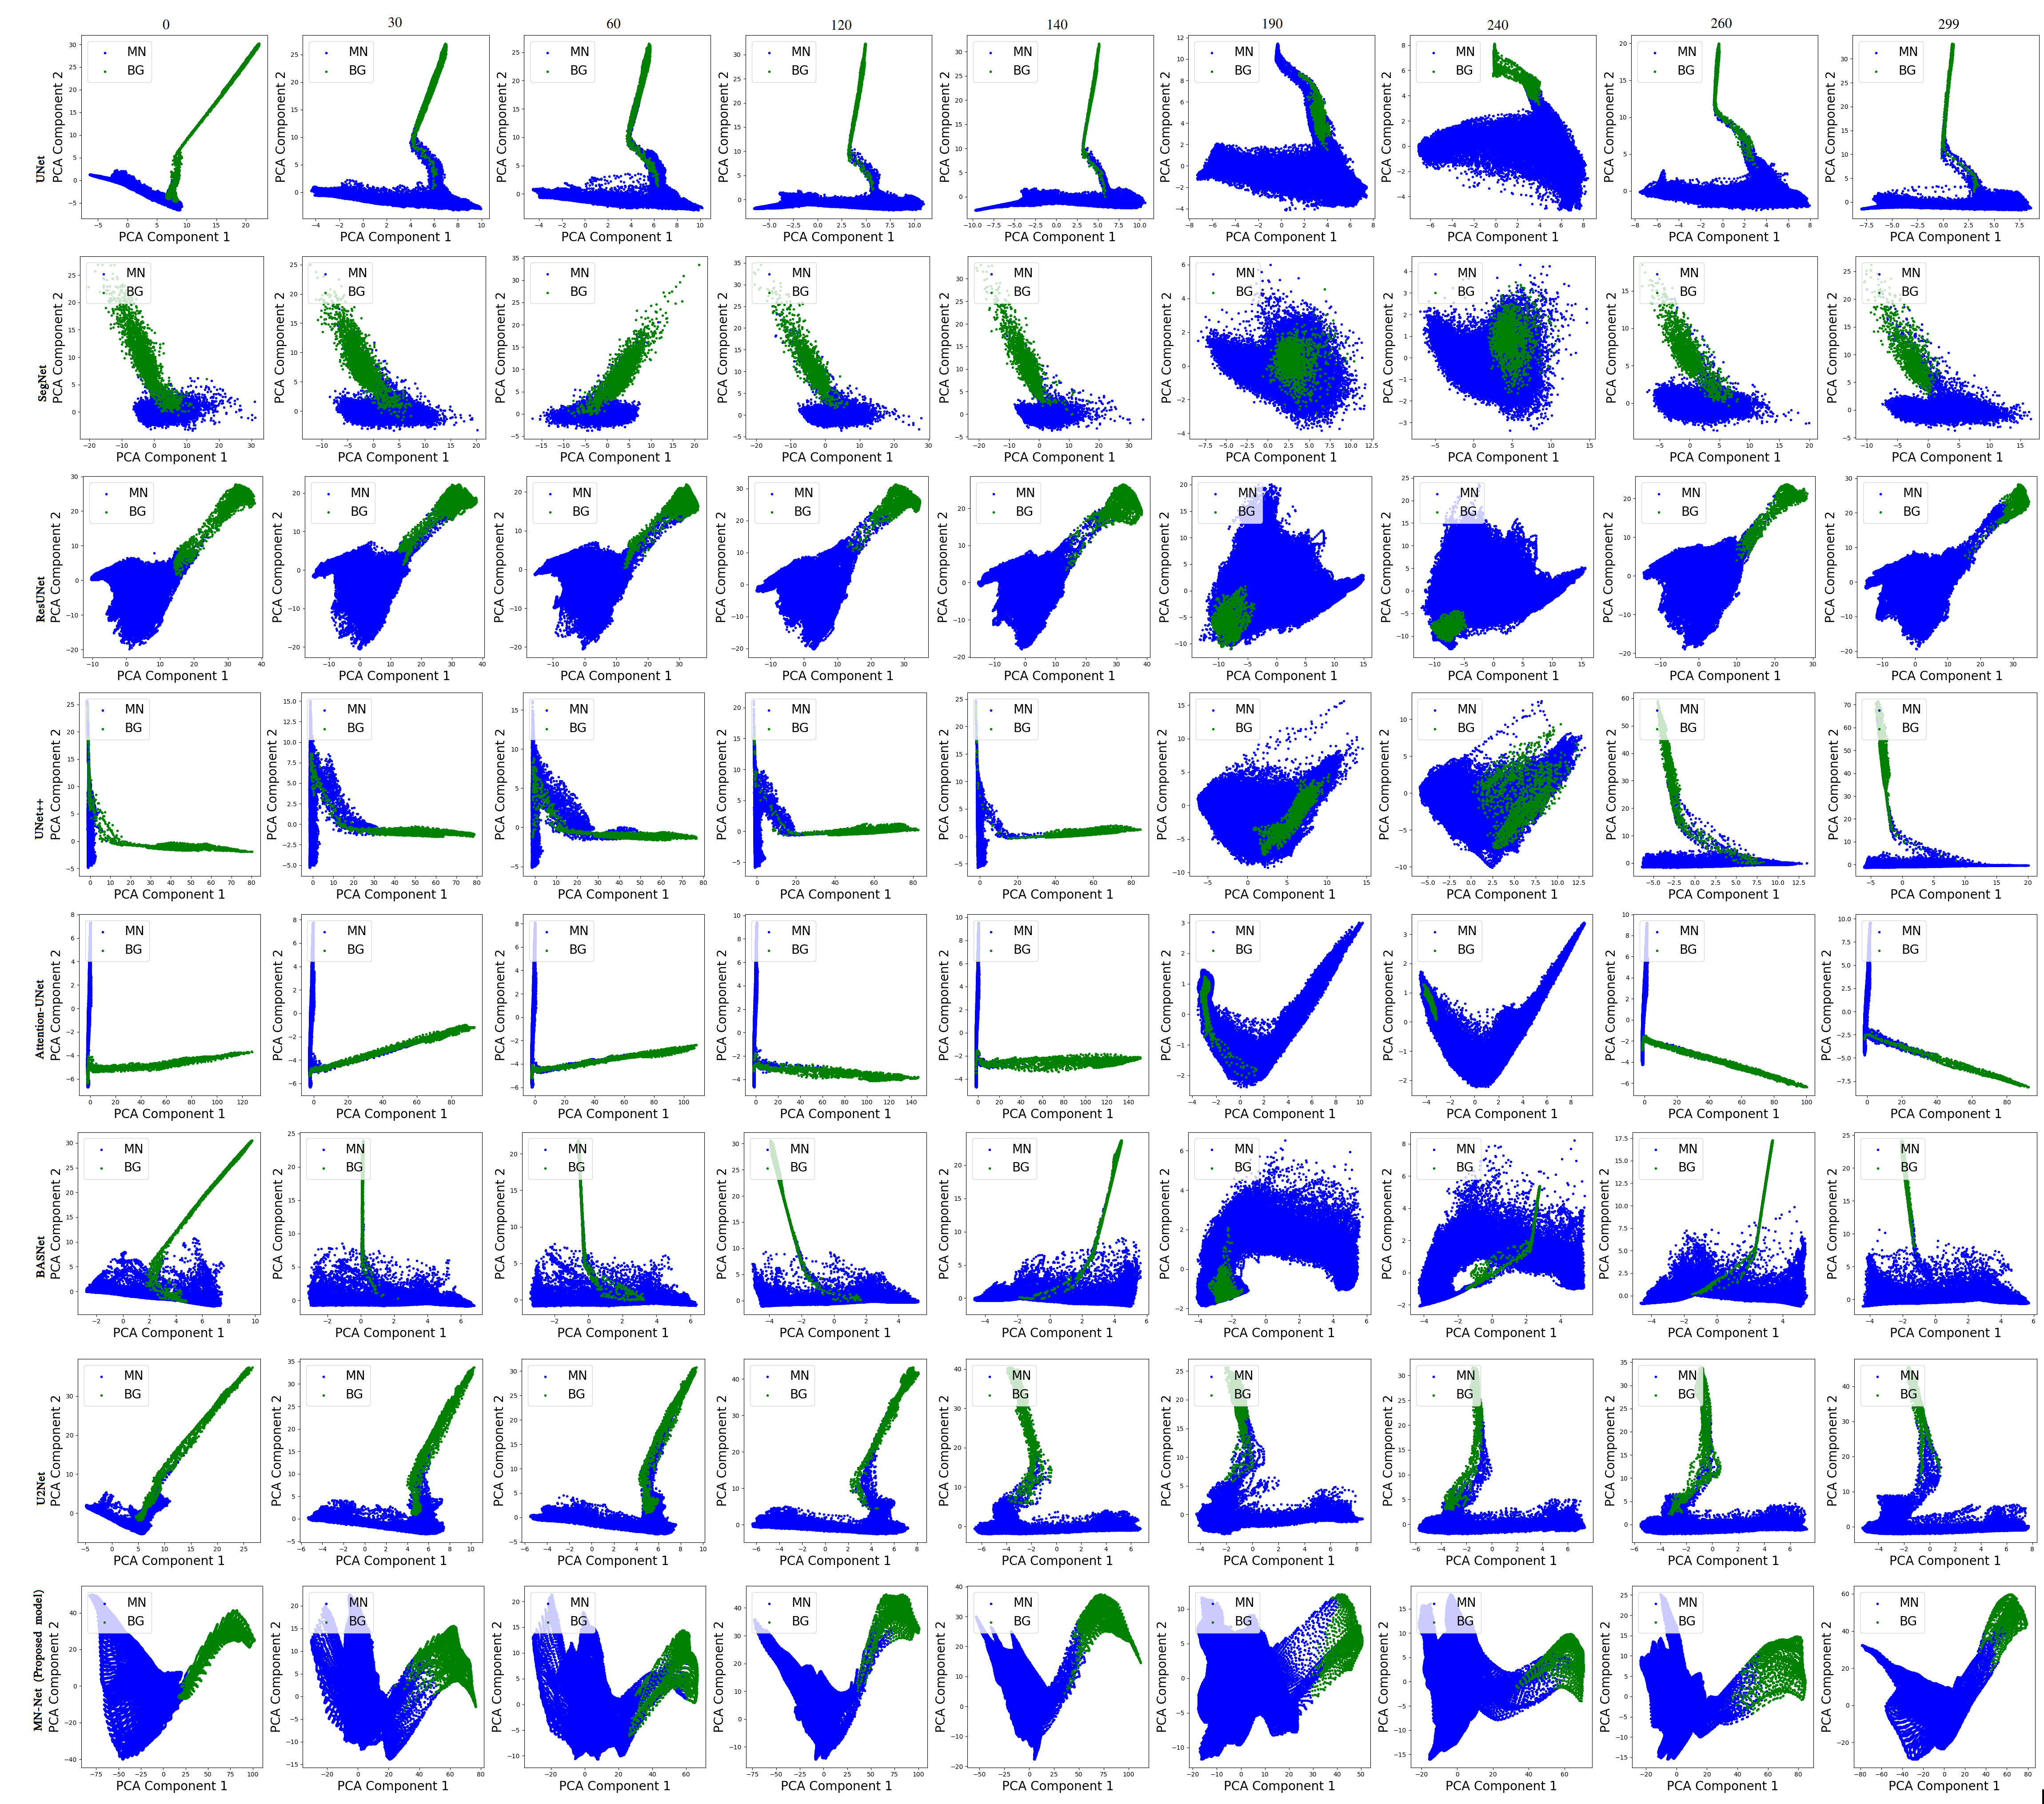
\includegraphics[width=1\textwidth]{Figure4}

\caption{Qualitative visualization of the learned feature representations for patient 1. The features extracted from the final encoder layer of each model were projected into two dimensions using PCA. Each point corresponds to a pixel classified as either background (blue) or median nerve (green). Compared with baseline models, MNSeg-Net exhibits clearer separation between the two classes, indicating more discriminative feature learning.} 
    
    \label{fig:pca_scatter_plots_updated}
\end{figure*}

\begin{figure*}[htbp]
    \centering
    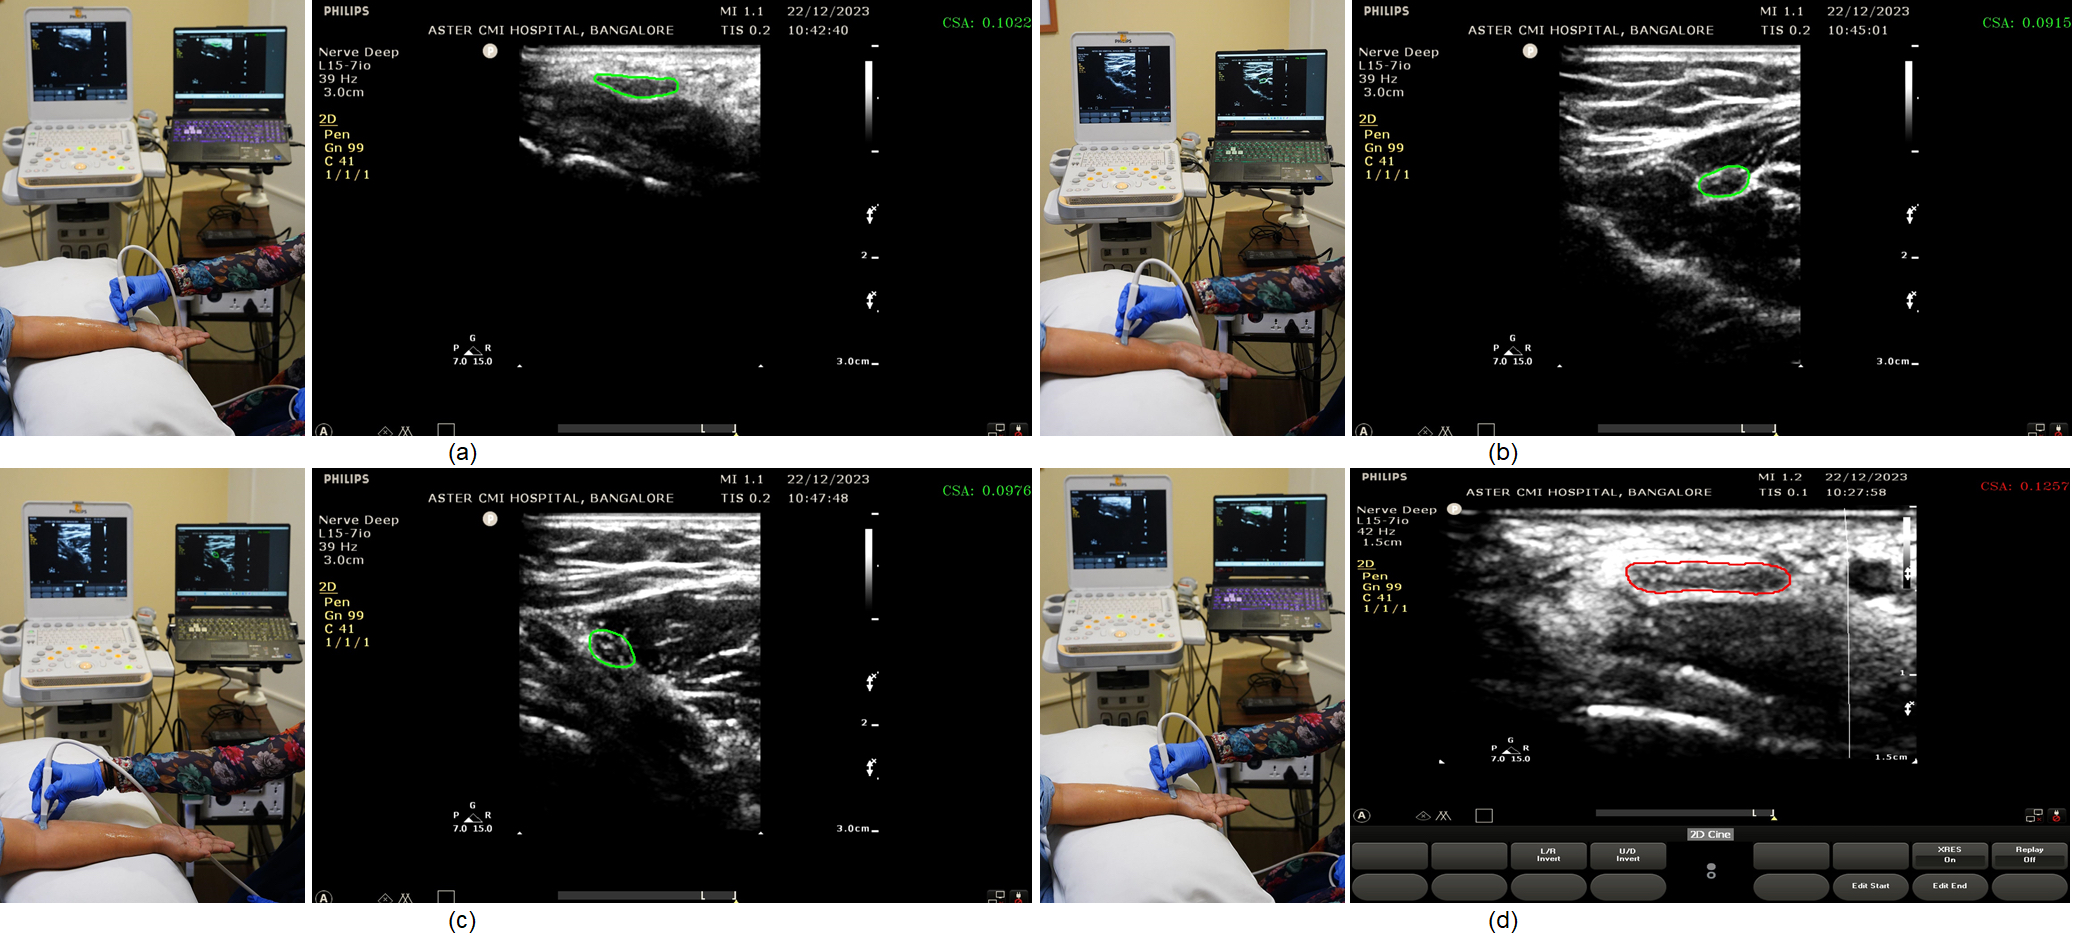
\includegraphics[width=1\textwidth]{Figure5}
    \caption{ (a), (b), and (c) represent sample images captured during real-time testing of wrist, forearm, and elbow scanning, shown alongside their corresponding median nerve segmentations and CSA in US frames. The CSA values are presented as $cm^{2}$. In addition, (d) illustrates a sample image in which the CSA surpassed the threshold of 0.12 $cm^{2}$ during wrist scanning. The CSA values are displayed in the top right corner of the ultrasound frame.  }
    \label{fig:real_time_screen_shots}
\end{figure*}

%\vspace{-15pt}




\begin{figure}[htbp]
    \centering
    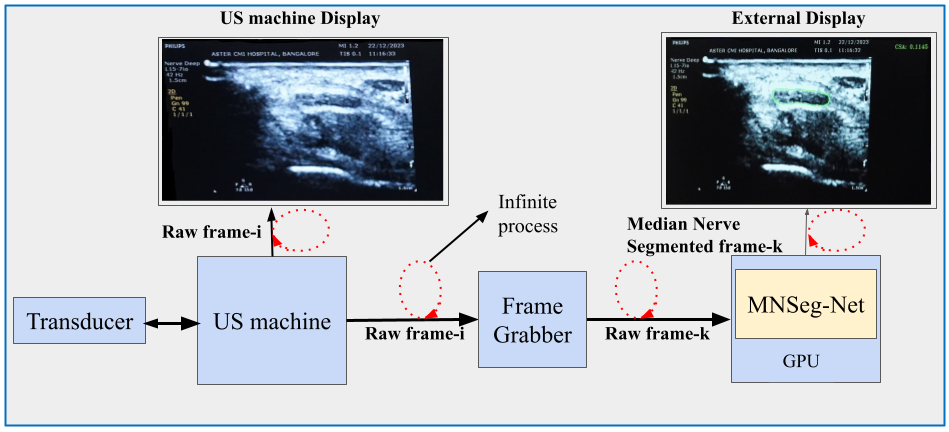
\includegraphics[width=\linewidth]{Figure6}
    \caption{Timeline diagram of the clinical workflow. The US transducer generates raw frames that are displayed on the ultrasound machine while simultaneously being captured via a frame grabber. The raw frames are sent to the GPU, where the proposed MNSeg-Net model processes them to generate segmented frames with CSA computation. These are displayed on an external screen, providing real-time quantitative and visual feedback alongside the ultrasound machine’s native display.}
    \label{fig:data_flow_diagram_of_clinical_setup}
\end{figure}




\subsection{Real-Time Setup}
The proposed median nerve segmentation model was deployed in a clinical setting using a customized desktop application. The real-time setup employed a frame grabber to capture the unprocessed video output of the ultrasound machine via a Digital Visual Interface (DVI). An AV.io frame grabber \cite{epiphan} captured the raw video output and converted it into serial frames, which were then transferred to a laptop (serving as an edge device) through a USB-B to USB-A interface. The laptop used these raw frames as input for the MNSeg-Net model, which was executed on its GPU using PyTorch inference. The model generated a segmentation mask for the median nerve, which was displayed as an overlay on the input frame along with the computed CSA on the laptop screen. This setup provided feedback to the operator in addition to the main screen of the ultrasound machine. Figure \ref{fig:clinical_setup} provides a comprehensive overview of the clinical setup, whereas Figure \ref{fig:data_flow_diagram_of_clinical_setup} illustrates the data flow/timeline diagram of the application. The development of this clinical setup was inspired by prior research \cite{van2018quantitative}. To the best of our knowledge, this is the first system to provide dual-screen real-time segmentation of the median nerve combined with quantitative CSA measurements during ultrasound scanning. To support this claim, a comprehensive literature review was performed. While some existing studies have addressed CSA measurement \cite{smerilli2022development} and others have proposed real-time segmentation techniques \cite{yeh2023real}, these methods were typically evaluated offline and not in clinical settings. The review—performed across PubMed, IEEE Xplore, and Google Scholar on 17-04-2025 using combinations of the keywords “median nerve,” “ultrasound,” “real-time segmentation,” “dual-screen interface,” and “CSA measurement”—confirmed that no prior work has unified real-time segmentation with quantitative CSA estimation in a dual-screen clinical system







\subsection{Feature Visualization}
\noindent
To qualitatively assess the discriminative capacity of the learned feature representations, feature embeddings were extracted from the final encoder layer of each model. Pixels corresponding to the median nerve and background were projected into two dimensions using principal component analysis (PCA). PCA was selected over non-linear techniques such as t-SNE because the embedding set for a single image frame contained 1,43,360 ($448 \times 320$) points in 64 dimensions, making t-SNE computationally expensive, sensitive to hyper parameters, and prone to overcrowding in large-scale settings. 

Feature representations were extracted from the sample images (subject-1) of each trained model.  Pixels corresponding to the median nerve and background were projected into two dimensions using principal component analysis (PCA) for data visualization. This allowed the 
higher-dimensional pixel embeddings in the segmentation map to be represented in a lower-dimensional space that is suitable for qualitative assessment.



\textcolor{black}{\subsection{Statistical Analysis}}

\textcolor{black}{The performance of the proposed MNSeg-Net was evaluated using a comprehensive statistical analysis based on the Dice Similarity Coefficient (DSC) and CSA. Since all segmentation models were evaluated on the same test images, paired statistical analyses were employed to account for within-sample dependence. Accordingly, paired $t$-tests were used to assess whether performance differences between MNSeg-Net and each benchmark model were statistically significant, following the classical formulation introduced by Student~\cite{student1908probable}. A significance threshold of $p < 0.05$ was adopted in accordance with widely accepted conventions in biomedical and clinical research. To quantify practical significance beyond statistical significance, effect sizes were computed using Cohen’s $d$. The magnitude of effects was interpreted using standardized thresholds for negligible ($|d| < 0.2$), small ($0.2 \leq |d| < 0.5$), moderate ($0.5 \leq |d| < 0.8$), and large ($|d| \geq 0.8$) effects, as proposed by Cohen~\cite{cohen1988statistical}. These effect size categories provide an interpretable measure of the magnitude of observed differences. To control for the increased risk of type~I error arising from multiple model comparisons, a one-way analysis of variance (ANOVA) was first conducted to assess whether overall differences existed among the evaluated models~\cite{fisher1925statistical}. When statistically significant differences were detected, Tukey’s Honestly Significant Difference (HSD) test was applied as a post-hoc analysis to identify specific model pairs exhibiting significant differences while controlling the family-wise error rate~\cite{tukey1949comparing}. } \textcolor{red}{ In addition, the mean difference was computed separately for DSC and CSA evaluation metrics to quantify the average paired deviation between models. For DSC, it represents the average paired difference between MNSeg-Net and the reference model, whereas for CSA it represents the average paired difference between clinician-annotated and model-predicted values. Mean differences were not aggregated across heterogeneous metrics with opposing optimization directions, and were used solely as descriptive measures of deviation.}


\textcolor{black}{\subsubsection{Equivalence Testing}}
\noindent
\textcolor{black}{In addition to conventional hypothesis testing, formal equivalence testing was performed using the two one-sided tests (TOST) procedure~\cite{schuirmann1987comparison} to assess whether observed differences lay within predefined margins of practical relevance. Equivalence testing was applied to both DSC and CSA measurements, reflecting distinct analytical objectives. For DSC-based model-to-model comparisons, equivalence margins of $\pm 0.01$, $\pm 0.03$, and $\pm 0.05$ were considered, representing increasingly relaxed criteria for practical similarity in segmentation performance commonly used in medical image analysis. For CSA evaluation, which represents an agreement analysis between model-predicted measurements and clinician-annotated reference values, equivalence testing was conducted at margins of  $\pm 0.5~\mathrm{mm}^2$, reflecting clinically meaningful tolerance ranges for median nerve CSA assessment. Equivalence was concluded only when the corresponding confidence intervals lay entirely within the specified equivalence margins.}

\section{Results}
%\vspace{-10pt}
\begin{table}[htbp]
  \centering
%  \caption{Performance comparison of deep learning models Utilised in this work (on 10 subjects test data)}

  \caption{Performance comparison of deep learning models evaluated on a 10-subject test dataset across two anatomical regions: the wrist and wrist-to-elbow. Evaluation metrics include DSC, Precision (Prec), Recall (Rec), and Hausdorff Distance (HD). $\uparrow$ indicates that higher values correspond to better performance, while $\downarrow$ indicates that lower values correspond to better performance.}
  \label{tab:model_performance}
  \scalebox{0.78}{

  \begin{tabular}{lcccccccc}
    \hline
    &\multicolumn{4}{c}{\textbf{At wrist region}} 
    &\multicolumn{4}{c}{\textbf{Wrist to Elbow}} \\
    \hline
    \textbf{Model} 
    &\textbf{DSC$\uparrow$} 
    &\textbf{Prec$\uparrow$} 
    &\textbf{Rec$\uparrow$} 
    &\textbf{HD$\downarrow$}  
    &\textbf{DSC$\uparrow$} 
    &\textbf{Prec$\uparrow$} 
    &\textbf{Rec$\uparrow$} 
    &\textbf{HD$\downarrow$}  \\
    \hline
    UNet & 0.943 & 0.940 & 0.946 &4.657 & 0.787 & 0.791 & 0.789  &14.421\\
    SegNet & 0.936 & 0.930 & 0.952 &4.852 &0.788  & 0.786 & 0.819 &16.428\\
    ResUnet & 0.945 & 0.947 & 0.945 &4.803 &0.781  & 0.804 & 0.786 &14.178\\
    Attention-UNet & 0.943 & 0.938 &\textbf{0.953} &7.720 &0.771  &0.786 &0.785 &14.221\\
    UNet++ & 0.942 &0.935 &\textbf{0.953} & 7.130 &0.755  &0.781 &0.766 &16.550\\
    BASNet & \textbf{0.947} & 0.955 & 0.942 &4.425& 0.823  & 0.825 & 0.838 &13.400\\
    U2Net-full & 0.945 & 0.957 & 0.937 &4.605 & \textbf{0.834}  & \textbf{0.844} & 0.840 &13.301\\
    %U2Net-light & 0.947 & 0.954 & 0.943&4.328 & 0.822  & 0.825 & 0.835 &13.701\\
    \textbf{\shortstack{MNSeg-Net\\(Proposed)}} & \textbf{0.947} & \textbf{0.965} &  0.945 &\textbf{4.177}& \textbf{0.834}  & 0.838 & \textbf{0.846} &\textbf{12.835}\\
    \hline
  \end{tabular}}
\end{table}

\subsection{Performance Comparison with Expert Annotation}
Table \ref{tab:model_specs} summarizes the models used in this study, including the parameter sizes, FLOPs per frame, training duration, and number of frames processed per second of each model. Table \ref{tab:model_performance} presents the average DSC, precision, recall, and HD across all frames for the ten test participants. All methods exhibited high accuracy and effectiveness in segmenting the median nerve at the wrist because of the consistent anatomy of the nerve and the lack of obstructing tissues. However, the performance of basic UNet-based methods noticeably declined further from the wrist towards the elbow, which is attributed to increased anatomical variability and surrounding structures, such as muscles and blood vessels. The proposed model, with its efficient subnetwork block design, demonstrated a superior ability to handle the complexities of localizing the median nerve in these regions. Table \ref{tab:patientwise_segmentation_and_statistical_comparison} displays all metrics for individual subjects (averaged across all frames) for the proposed model. Sample segmented images for subject-1 obtained using various models are shown in Fig. \ref{fig:sample_segmented_images_of_patient_1}. Each frame includes the computed CSA of the median nerve and DSC between the segmented output and expert annotation at the bottom. The results indicate that the proposed model outperforms existing deep learning models in segmenting the median nerve in ultrasound videos. As shown in Fig.~\ref{fig:pca_scatter_plots_updated}, the proposed MNSeg-Net model 
demonstrates a clearer separation between the pixel-embedding representations of 
median nerve and background compared to those of the other models.


\begin{table}[H]
\centering

\caption{
Comprehensive statistical comparison of segmentation models relative to the proposed MNSeg-Net (reference baseline) based on DSC. 
Mean differences and unadjusted p-values were computed using paired t-tests, and Cohen’s d values represent practical significance. 
Effect size interpretation: N = Negligible (\(d < 0.2\)), S = Small (\(0.2 \leq d < 0.5\)), 
M = Moderate (\(0.5 \leq d < 0.8\)), and L = Large (\(d \geq 0.8\)). An asterisk (*) denotes a statistically significant difference from MNSeg-Net at \( p < 0.05 \) after Tukey correction.
}

\scalebox{0.75}{
\begin{tabular}{lcccccc}
\hline
\textbf{Model} 
& \textbf{\shortstack{Mean\\Difference}} 
& \textbf{\shortstack{p-value\\(paired t-test)}} 
& \textbf{\shortstack{Effect size\\Cohen’s d}} 
& \textbf{\shortstack{p-value\\(Tukey adj)}} 
& \textbf{\shortstack{95\% CI\\(Lower)}} 
& \textbf{\shortstack{95\% CI\\(Upper)}} \\
\hline

UNet$^{*}$ 
& 0.069 
& $8.70 \times 10^{-29}$ 
& 0.289 (S) 
& 0.000 
& -0.088 
& -0.049 \\

SegNet$^{*}$ 
& 0.034 
& $6.56 \times 10^{-10}$ 
& 0.160 (N) 
& 0.000 
& -0.053 
& -0.015 \\

ResUNet$^{*}$ 
& 0.054 
& $8.67 \times 10^{-19}$ 
& 0.229 (S) 
& 0.000 
& -0.073 
& -0.034 \\

Attention-UNet$^{*}$ 
& 0.063 
& $3.41 \times 10^{-23}$ 
& 0.257 (S) 
& 0.000 
& 0.044 
& 0.082 \\

UNet++$^{*}$ 
& 0.079 
& $4.06 \times 10^{-33}$ 
& 0.312 (S) 
& 0.000 
& -0.098 
& -0.059 \\

BASNet 
& 0.011 
& $4.00 \times 10^{-2}$ 
& 0.053 (N) 
& 0.738 
& -0.009 
& 0.030 \\

U2Net 
& -0.001 
& $9.11 \times 10^{-1}$ 
& -0.003 (N) 
& 1.000 
& -0.019 
& 0.020 \\

\hline
\end{tabular}}
\label{tab:stats_analysis_on_old_data_dsc}
\end{table}

 
\begin{table}[H]
\centering

\caption{
Comprehensive statistical comparison of model-predicted CSA values relative to clinician-annotated CSA\textsubscript{Act} (reference baseline). 
Mean differences and unadjusted p-values were computed using paired t-tests, and Cohen’s d values represent practical significance. 
Effect size interpretation: N = Negligible (\(d < 0.2\)), S = Small (\(0.2 \leq d < 0.5\)), 
M = Moderate (\(0.5 \leq d < 0.8\)), and L = Large (\(d \geq 0.8\)). 
An asterisk (*) denotes a statistically significant difference from CSA\textsubscript{Act} at \( p < 0.05 \) after Tukey correction.
}

\scalebox{0.75}{
\begin{tabular}{lcccccc}
\hline
\textbf{Model} 
& \textbf{\shortstack{Mean Diff\\(CSA\textsubscript{Act} - CSA\textsubscript{Cal})}} 
& \textbf{\shortstack{p-value\\(paired t-test)}} 
& \textbf{\shortstack{Effect size\\Cohen’s d}} 
& \textbf{\shortstack{p-value\\(Tukey adj)}} 
& \textbf{\shortstack{95\% CI\\(Lower)}} 
& \textbf{\shortstack{95\% CI\\(Upper)}} \\
\hline

UNet$^{*}$ 
& 0.538 
& $1.34 \times 10^{-13}$ 
& 0.192 (N) 
& 0.000 
& 0.321 
& 0.755 \\

SegNet 
& -0.186 
& $3.80 \times 10^{-3}$ 
& -0.075 (N) 
& 0.168 
& -0.403 
& 0.031 \\

ResUNet$^{*}$ 
& 0.659 
& $8.57 \times 10^{-23}$ 
& 0.255 (S) 
& 0.000 
& 0.442 
& 0.876 \\

Attention-UNet$^{*}$ 
& 0.694 
& $7.40 \times 10^{-22}$ 
& 0.249 (S) 
& 0.000 
& 0.477 
& 0.911 \\

UNet++$^{*}$ 
& 0.977 
& $3.99 \times 10^{-39}$ 
& 0.341 (S) 
& 0.000 
& 0.760 
& 1.194 \\

BASNet 
& -0.054 
& $3.41 \times 10^{-1}$ 
& -0.025 (N) 
& 0.999 
& -0.271 
& 0.163 \\

U2Net 
& 0.105 
& $3.88 \times 10^{-2}$ 
& 0.053 (N) 
& 0.882 
& -0.322 
& 0.112 \\

MNSeg-Net 
& -0.081 
& $1.14 \times 10^{-1}$ 
& -0.041 (N) 
& 0.976 
& -0.298 
& 0.136 \\

\hline
\end{tabular}}
\label{tab:stats_analysis_on_old_data_csa}

\end{table}








\subsection{Statistical Analysis}
\subsubsection{DSC-based Evaluation:}
Table~\ref{tab:stats_analysis_on_old_data_dsc} summarizes the paired t-test results for DSC. All models, except U2Net, demonstrated statistically significant differences compared to MNSeg-Net (\(p < 0.05\)), with p-values of \(8.70 \times 10^{-29}\) for UNet, \(6.56 \times 10^{-10}\) for SegNet, and \(4.06 \times 10^{-33}\) for UNet++. Despite being statistically significant, the effect sizes were generally small (e.g., 0.160 for SegNet, 0.229 for ResUNet, and 0.312 for UNet++), suggesting a limited practical impact. U2Net exhibited a negligible mean difference of –0.001 and an effect size of –0.003, indicating that its performance was statistically and practically similar to that of MNSeg-Net.

\subsubsection{CSA-based Evaluation:}
As shown in Table~\ref{tab:stats_analysis_on_old_data_csa}, MNSeg-Net produced a non-significant p-value of \(1.14 \times 10^{-1}\) and a negligible effect size of –0.041 compared with the clinician-annotated CSA\textsubscript{Act}, demonstrating strong alignment with the clinical ground truth. Similarly, BASNet exhibited a non-significant difference (\(p = 3.41 \times 10^{-1}\), \(d = -0.025\)). Conversely, UNet (\(p = 1.34 \times 10^{-13}\), \(d = 0.192\)), ResUNet (\(p = 8.57 \times 10^{-23}\), \(d = 0.255\)), and UNet++ (\(p = 3.99 \times 10^{-39}\), \(d = 0.341\)) showed significant difference and moderate effect sizes, suggesting notable deviations from CSA\textsubscript{Act}.



\subsubsection{Multiple Comparison Correction}\label{multiple_comparison_correction} 

To address the risk of type I error arising from multiple comparisons, a one-way ANOVA followed by Tukey’s HSD test was conducted. The ANOVA on the DSC yielded a highly significant result (\(p = 1.72 \times 10^{-80} < 0.05\)), indicating statistically significant differences among the evaluated models. Tukey’s HSD analysis (Table~6) showed that MNSeg-Net significantly outperformed UNet ($p \approx 1 \times 10^{-308} < 0.05$), SegNet ($p \approx 1 \times 10^{-308} < 0.05$), ResUNet ($p \approx 1 \times 10^{-308} < 0.05$), UNet++ ($p \approx 1 \times 10^{-308} < 0.05$), and Attention-UNet ($p \approx 1 \times 10^{-308} < 0.05$). In contrast, BASNet (\(p = 0.738\)) and U2Net (\(p = 1.000\)) did not exhibit statistically significant differences, confirming comparable performance.

For CSA, ANOVA similarly revealed significant group differences (\(p = 1.05 \times 10^{-134}< 0.05\)). Tukey’s HSD results (Table~7) indicated a significant overestimation by UNet ($p \approx 1 \times 10^{-308} < 0.05$), ResUNet ($p \approx 1 \times 10^{-308} < 0.05$), UNet++ ($p \approx 1 \times 10^{-308} < 0.05$), and Attention-UNet ($p \approx 1 \times 10^{-308} < 0.05$). In contrast, MNSeg-Net (\(p = 0.9761\)), BASNet (\(p = 0.9988\)), SegNet (\(p = 0.1678\)), and U2Net (\(p = 0.8819\)) did not differ significantly from CSA\textsubscript{Act}, with MNSeg-Net exhibiting the lowest mean deviation of $-0.0806$.

Overall, MNSeg-Net demonstrated strong statistical and practical agreement with expert annotations, particularly in CSA estimation, where it showed minimal deviation from the clinician-provided ground truth. Furthermore, it achieved consistently high DSC performance and statistically validated improvements over several baseline models, while appropriately controlling for type I error through multiple-comparison correction.
 

%---------------------------------
% \begin{table}[H] 
%     \centering
%     \caption{
%         Statistical comparison of segmentation models with the proposed MNSeg-Net (used as a reference) based on the ((DSC). 
%         Mean differences and p-values were calculated using paired t-tests. Cohen’s d values represent effect sizes.
%         (*) indicates a statistically significant difference from MNSeg-Net at \( p < 0.05 \). Effect size abbreviations: N = Negligible (\(d < 0.2\)), S = Small (\(0.2 \leq d < 0.5\)), M = Moderate (\(0.5 \leq d < 0.8\)), L = Large (\(d \geq 0.8\)). MNSeg-Net consistently outperformed UNet, ResUNet, Attention-UNet, UNet++, SegNet, and BASNet, with statistically significant differences, 
% while showing no significant difference compared to U2Net.}
    

    
%     \scalebox{0.8}{
%     \begin{tabular}{lcccc}
% \hline
%         \textbf{Model} & \textbf{\shortstack{Mean\\Difference}} & \textbf{\shortstack{p-value\\(paired t-test)}} & \textbf{\shortstack{Effect Size\\(Cohen's d)}} & \textbf{Significant} \\
% \hline
%         UNet            & 0.069$^*$  & \(8.70 \times 10^{-29}\)$^*$  & 0.289 (S)$^*$   & Yes \\
%         SegNet          & 0.034$^*$  & \(6.56 \times 10^{-10}\)$^*$  & 0.160 (N)    & Yes \\
%         ResUNet         & 0.054$^*$  & \(8.67 \times 10^{-19}\)$^*$  & 0.229 (S)$^*$   & Yes \\
%         Attention-UNet  & 0.063$^*$  & \(3.41 \times 10^{-23}\)$^*$  & 0.257 (S)$^*$   & Yes \\
%         UNet++          & 0.079$^*$  & \(4.06 \times 10^{-33}\)$^*$  & 0.312 (S)$^*$   & Yes \\
%         BASNet          & 0.011$^*$  & \(4.00 \times 10^{-2}\)$^*$   & 0.053 (N)    & Yes \\
%         U2Net           & -0.001  & \(9.11 \times 10^{-1}\)     & -0.003 (N)   & No \\

% \hline
%     \end{tabular}}
%     \label{tab:stats_analysis_on_old_data_dsc}
% \end{table}



% \begin{table}[H]
% \centering
% \caption{Tukey’s HSD test results comparing dice scores of MNSeg-Net with other segmentation models. The table includes mean differences, 95\% confidence intervals (CI), adjusted p-values, and statistical significance at \( p < 0.05 \). MNSeg-Net achieved higher DSC values than all models, with statistically significant differences for all except BASNet and U2Net, highlighting its superior segmentation performance.}


% {\scalebox{0.8}{
% \begin{tabular}{lccccc}
% \hline
% \textbf{Model} & \textbf{\shortstack{Mean\\Difference}} & \textbf{\shortstack{p-value\\Tukey's HSD}} &  \textbf{95\% CI Lower} & \textbf{95\% CI Upper} & \textbf{Significant} \\
% \hline
% UNet                  & -0.069 & 0.000 & -0.088 & -0.049 & Yes \\
% SegNet                & -0.034 & 0.000 & -0.053 & -0.015 & Yes \\
% ResUNet               & -0.054 & 0.000 & -0.073 & -0.034 & Yes \\
% Attention-UNet        &  0.063 & 0.000 &  0.044 &  0.082 & Yes \\
% UNet++                & -0.079 & 0.000 & -0.098 & -0.059 & Yes \\
% BASNet                &  0.011 & 0.738 & -0.009 &  0.030 & No \\
% U2Net                 &  0.001 & 1.000 & -0.019 &  0.020 & No \\
% \hline
% \end{tabular}}

% \label{tab:tukey_dsc_models_for_old_data}
% \end{table}}


















































% \begin{table}[H]
%     \centering
%     \caption{Statistical comparison of predicted CSA values from different models with the clinician-annotated CSA\textsubscript{Act}. 
%         The table includes the mean differences, p-values from paired t-tests, and Cohen’s d effect sizes. 
%         (*) indicates a statistically significant difference from CSA\textsubscript{Act} at \( p < 0.05 \). Effect size abbreviations: N = Negligible (\(d < 0.2\)), S = Small (\(0.2 \leq d < 0.5\)), M = Moderate (\(0.5 \leq d < 0.8\)), L = Large (\(d \geq 0.8\)).  MNSeg-Net achieved the closest agreement with clinician-annotated CSA values, with no statistically significant difference, whereas most other models showed significant deviations.
%         }
%     \scalebox{0.8}{
%     \begin{tabular}{lcccc}
% \hline
%         \textbf{Model} & \textbf{\shortstack{Mean Difference\\(CSA\textsubscript{Act} - CSA\textsubscript{Cal})}} 
%         & \textbf{\shortstack{p-value\\(paired t-test)}} & \textbf{\shortstack{Effect Size\\(Cohen's d)}} & \textbf{Significant} \\
% \hline
%         UNet            & 0.538$^*$  & \(1.34 \times 10^{-13}\)$^*$ & 0.192 (N)  & Yes \\
%         SegNet          & -0.186$^*$ & \(3.80 \times 10^{-3}\)$^*$  & -0.075 (N) & Yes \\
%         ResUNet         & 0.659$^*$  & \(8.57 \times 10^{-23}\)$^*$ & 0.255 (S)$^*$ & Yes \\
%         Attention-UNet  & 0.694$^*$  & \(7.40 \times 10^{-22}\)$^*$ & 0.249 (S)$^*$ & Yes \\
%         UNet++           & 0.977$^*$ & \(3.99 \times 10^{-39}\)$^*$                 & 0.341 (S)$^*$    &Yes \\
%         BASNet          & -0.054  & \(3.41 \times 10^{-1}\)    & -0.025 (N) & No \\
%         U2Net           & 0.105$^*$  & \(3.88 \times 10^{-2}\)$^*$  & 0.053 (N)  & Yes \\
%         MNSeg-Net       & -0.081  & \(1.14 \times 10^{-1}\)    & -0.041 (N) & No \\
        
% \hline
%     \end{tabular}}



    
%     \label{tab:stats_analysis_on_old_data_csa}
% \end{table}



% \begin{table}[H]
% \caption{Tukey’s HSD test results comparing model-predicted CSA values with clinician-annotated CSA\textsubscript{Act}. 
% The table includes mean differences, confidence intervals (CI), and significance status based on \( p < 0.05 \). MNSeg-Net showed no statistically significant difference from clinician-annotated CSA values, indicating close agreement with the ground truth, whereas UNet, ResUNet, Attention-UNet, and UNet++ exhibited significant deviations.
% }
% \centering
% \scalebox{0.8}{
% \begin{tabular}{lccccc}
% \hline
% \textbf{Model} & \textbf{\shortstack{Mean\\Difference}} & \textbf{\shortstack{p-value\\(Tukey's HSD)}} & \textbf{95\% CI Lower} & \textbf{95\% CI Upper} & \textbf{Significant} \\
% \hline
% UNet & 0.538 & 0.000 & 0.321 & 0.755 & Yes \\
% SegNet & -0.186 & 0.168 & -0.403 & 0.031 & No \\
% ResUNet & 0.659 & 0.000 & 0.442 & 0.876 & Yes \\
% Attention-UNet & 0.694 & 0.000 & 0.477 & 0.911 & Yes \\
% UNet++ & 0.977 & 0.000 & 0.760 & 1.194 & Yes \\
% BASNet & -0.054 & 0.999 & -0.271 & 0.163 & No \\
% U2Net & -0.105 & 0.882 & -0.322 & 0.112 & No \\
% MNSeg-Net & -0.081 & 0.976 & -0.298 & 0.136 & No \\
% \hline
% \end{tabular}}

% \label{tab:tukey_csa_models_for_old_data}
% \end{table}





%------------------












%---------------------------




















\begin{table}[htbp]
\centering
\caption{Two One-Sided Tests (TOST) equivalence test results for DSC scores of MNSeg-Net versus other models. The table reports mean differences with 95\% confidence intervals and equivalence decisions at margins $\pm$0.01, $\pm$0.03, and $\pm$0.05. MNSeg-Net was statistically equivalent to U2Net at all tested margins, BASNet at $\pm$0.03 and $\pm$0.05, and SegNet at $\pm$0.05 only. No equivalence was found with UNet, ResUNet, Attention-UNet, or UNet++.}

\label{tab:f1_tost_equivalence_summary}
\renewcommand{\arraystretch}{1.15}
\scalebox{0.7}{%
\begin{tabular}{lcccccc}
\hline
\textbf{\shortstack{Model}} & \textbf{\shortstack{Mean\\Difference}} & \textbf{95\% CI Lower} & \textbf{95\% CI Upper} 
& \textbf{\shortstack{Equivalent\\ (margin=0.01)}} 
& \textbf{\shortstack{Equivalent\\ (margin=0.03)}} 
& \textbf{\shortstack{Equivalent\\ (margin=0.05)}} \\
\hline
UNet           & $0.0686$  & $0.0605$  & $0.0768$ & No  & No  & No  \\
SegNet         & $0.0340$  & $0.0269$  & $0.0410$ & No  & No  & Yes \\
ResUNet        & $0.0537$  & $0.0454$  & $0.0621$ & No  & No  & No  \\
Attention-UNet & $0.0629$  & $0.0541$  & $0.0717$ & No  & No  & No  \\
UNet++         & $0.0786$  & $0.0694$  & $0.0878$ & No  & No  & No  \\
BASNet         & $0.0107$  & $0.0039$  & $0.0176$ & No  & Yes & Yes \\
U2Net          & $-0.0006$ & $-0.0066$ & $0.0055$ & Yes & Yes & Yes \\
\hline
\end{tabular}%
}
\end{table}




\begin{table}[htbp]
\centering
% \caption{TOST equivalence test results for CSA (actual vs. computed) at margin $\pm$0.5, indicating that the proposed MNSeg-Net,SegNet, BASNet, and U2Net achieved equivalence, while UNet, ResUNet, Attention-UNet, and UNet++ did not.}

\caption{TOST equivalence test results for CSA (actual vs. computed) at margin $\pm$0.5. The proposed MNSeg-Net, SegNet, BASNet, and U2Net models met the equivalence criterion, whereas UNet, ResUNet, Attention-UNet, and UNet++ did not. At the equivalence margin of $\pm$0.5, MNSeg-Net, SegNet, BASNet, and U2Net demonstrated statistical equivalence with the clinician-annotated CSA values. In contrast, UNet, ResUNet, Attention-UNet, and UNet++ did not achieve statistical equivalence under this criterion.}


\label{tab:csa_tost_equivalence_05}
\scalebox{0.8}{
\begin{tabular}{lcccc}
\hline
\textbf{Model} & \textbf{Mean Difference} & \textbf{95\% CI Lower} & \textbf{95\% CI Upper} & \textbf{Equivalent ($\pm$0.5)} \\
\hline
% u2net-p & -0.0661 & -0.1323 & 0.0002 & Yes \\
UNet & 0.5383 & 0.4178 & 0.6588 & No \\
SegNet & -0.1859 & -0.2840 & -0.0878 & Yes \\
ResUNet & 0.6595 & 0.5582 & 0.7609 & No \\
Attention-UNet & 0.6945 & 0.5808 & 0.8083 & No \\
UNet++ & 0.9778 & 0.8573 & 1.0983 & No \\
BASNet & -0.0540 & -0.1324 & 0.0244 & Yes \\
U2Net & 0.1046 & 0.0386 & 0.1705 & Yes \\
MNSeg-Net & -0.0807 & -0.1491 & -0.0123 & Yes \\
\hline
\end{tabular}}
\end{table}



\begin{table}[htbp]
\centering
{\color{red}
% \caption{TOST equivalence results for MNSeg-Net vs U2Net (frame-level analysis).}

\caption{TOST equivalence analysis of frame-level DSC between MNSeg-Net and U2Net. It reports the mean difference, 95\% confidence interval, and equivalence decisions under predefined DSC margins.}

\label{tab:u2net_tost_equivalence_on_dsc}
\renewcommand{\arraystretch}{1.15}
\scalebox{0.7}{%
\begin{tabular}{cccccc}
\hline
\textbf{\shortstack{Mean\\Difference}} 
& \textbf{95\% CI Lower} 
& \textbf{95\% CI Upper} 
& \textbf{\shortstack{Equivalent\\ (margin=0.01)}} 
& \textbf{\shortstack{Equivalent\\ (margin=0.03)}} 
& \textbf{\shortstack{Equivalent\\ (margin=0.05)}} \\
\hline
$-0.0006$ & $-0.0066$ & $0.0055$ & Yes & Yes & Yes \\
\hline
\end{tabular}}
}
\end{table}

 

 

\begin{table}[htbp]
\centering
\textcolor{red}{
\caption{TOST equivalence analysis of frame-level CSA estimates between MNSeg-Net and U2Net. It reports the mean difference, 95\% confidence interval, and equivalence decisions under clinically defined CSA margins (in mm$^2$).}
\label{tab:u2net_tost_equivalence_on_csa}
\renewcommand{\arraystretch}{1.15}
\scalebox{0.8}{
\begin{tabular}{cccccc}
\hline
\textbf{\shortstack{Mean\\Difference}} 
& \textbf{95\% CI Lower} 
& \textbf{95\% CI Upper} 
& \textbf{\shortstack{Equivalent\\ (margin=0.1)}} 
& \textbf{\shortstack{Equivalent\\ (margin=0.3)}} 
& \textbf{\shortstack{Equivalent\\ (margin=0.5)}} \\
\hline
$0.1852$ & $0.1359$ & $0.2346$ & No & Yes & Yes \\
\hline
\end{tabular}}}
\end{table}



{\subsubsection{TOST Equivalence Analysis of DSC and CSA}}

\noindent
The results, summarized in Table~\ref{tab:f1_tost_equivalence_summary}, indicated that U2Net was statistically equivalent to MNSeg-Net even at the strictest margin of $\pm$0.01, while BASNet became equivalent at the wider margin of $\pm$0.02. At the broadest margin of $\pm$0.05, equivalence was observed for U2Net, BASNet, and SegNet. In contrast, UNet consistently failed to meet equivalence criteria across all tested margins, highlighting a significant performance gap compared to MNSeg-Net. Similarly, Attention-UNet, ResUNet, and UNet++ did not achieve equivalence within these margins, despite showing competitive DSC scores. These findings reinforce that MNSeg-Net exhibits performance that is statistically indistinguishable from several advanced architectures under practical equivalence thresholds, while maintaining superiority over models such as UNet.

\noindent
The results, presented in Table~\ref{tab:csa_tost_equivalence_05}, show that at the narrowest margin of $\pm$0.1, none of the models achieved equivalence with the actual CSA, suggesting that small differences persist at very strict thresholds. When the margin was relaxed to $\pm$0.2, BASNet satisfied the equivalence criteria, indicating its predictions were statistically indistinguishable from the ground truth within this tolerance. At $\pm$0.5, a broader set of models—including U2Net, MNSeg-Net, BASNet, and SegNet—achieved equivalence, while UNet continued to show significant deviation. At the widest tested margin of $\pm$1.0, all models except UNet demonstrated equivalence with the actual CSA. These findings highlight that while certain models such as U2Net and BASNet align closely with the actual CSA even under tighter thresholds, UNet consistently fails to meet equivalence criteria, reflecting its systematic bias in CSA estimation.




 \begin{table}[H]
\centering
\caption{Subject-wise evaluation of the proposed MNSeg-Net model from wrist to elbow, including segmentation metrics (DSC, precision, recall, HD) and a statistical comparison between the predicted CSA values from MNSeg-Net (CSA\textsubscript{Cal}) and clinician-annotated CSA values (CSA\textsubscript{Act}). Paired t-tests, Cohen’s \(d\) effect sizes, mean differences, and confidence intervals were computed across 300 image frames per subject to assess the clinical reliability of the MNSeg-Net. Equivalence was assessed using the TOST procedure with predefined margins of \(\pm 0.5~\mathrm{mm}^2\). Asterisks (*) denote statistically significant differences (\(p < 0.05\)). Effect size categories: N = Negligible (\(d < 0.2\)), S = Small (\(0.2 \leq d < 0.5\)), M = Moderate (\(0.5 \leq d < 0.8\)), L = Large (\(d \geq 0.8\)).}

\scalebox{0.63}{
\begin{tabular}{ccccccccccccc}
\hline
\textbf{\shortstack{Subject\\ID}} 
& \textbf{DSC$\uparrow$} 
& \textbf{Prec$\uparrow$} 
& \textbf{Rec$\uparrow$} 
& \textbf{HD$\downarrow$}
& \textbf{CSA\textsubscript{Cal}} 
& \textbf{CSA\textsubscript{Act}} 
& \textbf{\shortstack{t-test \\p-value}} 
& \textbf{\shortstack{Cohen's \(d\)\\(N/S/M/L)}} 
& \textbf{\shortstack{Mean\\Difference}} 
& \textbf{\textcolor{black}{\shortstack{95\% CI\\Lower}}} 
& \textbf{\textcolor{black}{\shortstack{95\% CI\\Upper}}} 
& \textbf{\textcolor{black}{\shortstack{Equivalent\\(\(\pm 0.5\))}}} \\
\hline
1  & 0.891 & 0.854 & 0.896 & 8.993  & 8.297 & 7.937 & 0.0015$^*$ & 0.254 (S) & 0.360 & \textcolor{black}{0.198} & \textcolor{black}{0.522} & \textcolor{black}{Yes} \\
2  & 0.898 & 0.893 & 0.913 & 7.081  & 8.319 & 8.126 & 0.0124$^*$ & 0.145 (N) & 0.193 & \textcolor{black}{0.045} & \textcolor{black}{0.341} & \textcolor{black}{Yes} \\
3  & 0.786 & 0.812 & 0.776 & 19.909 & 8.666 & 9.278 & 0.0000$^*$ & -0.289 (S) & -0.612 & \textcolor{black}{-0.808} & \textcolor{black}{-0.416} & \textcolor{black}{No} \\
4  & 0.704 & 0.695 & 0.738 & 23.511 & 10.140 & 9.292 & 0.0000$^*$ & 0.327 (S) & 0.849 & \textcolor{black}{0.618} & \textcolor{black}{1.080} & \textcolor{black}{No} \\
5  & 0.840 & 0.807 & 0.900 & 11.222 & 9.539 & 8.484 & 0.0000$^*$ & 0.501 (M) & 1.055 & \textcolor{black}{0.826} & \textcolor{black}{1.284} & \textcolor{black}{No} \\
6  & 0.890 & 0.888 & 0.899 & 8.005  & 8.499 & 8.364 & 0.0457$^*$ & 0.116 (N) & 0.136 & \textcolor{black}{0.006} & \textcolor{black}{0.266} & \textcolor{black}{Yes} \\
7  & 0.878 & 0.880 & 0.886 & 9.705  & 8.849 & 8.860 & 0.8963    & -0.008 (N) & -0.011 & \textcolor{black}{-0.141} & \textcolor{black}{0.119} & \textcolor{black}{Yes} \\
8  & 0.768 & 0.773 & 0.783 & 14.741 & 7.404 & 7.404 & 0.9987    & -0.000 (N) & -0.000 & \textcolor{black}{-0.132} & \textcolor{black}{0.132} & \textcolor{black}{Yes} \\
9  & 0.818 & 0.845 & 0.810 & 14.940 & 6.791 & 7.023 & 0.0253$^*$ & -0.130 (N) & -0.233 & \textcolor{black}{-0.416} & \textcolor{black}{-0.050} & \textcolor{black}{Yes} \\
10 & 0.888 & 0.932 & 0.861 & 10.244 & 8.776 & 9.705 & 0.0000$^*$ & -0.501 (M) & -0.928 & \textcolor{black}{-1.124} & \textcolor{black}{-0.732} & \textcolor{black}{No} \\
\hline
\end{tabular}}
\label{tab:patientwise_segmentation_and_statistical_comparison}

\end{table}


 



\subsubsection{Subject-wise Statistical Analysis} 
\label{sec:Patient_wise_Statistical_Analysis}

A comprehensive subject-wise statistical analysis was performed on Dataset-1 to compare the clinician-annotated CSA (CSA\textsubscript{Act}) with the MNSeg-Net-predicted CSA (CSA\textsubscript{Cal}). For each subject, paired t-tests, mean differences, and effect sizes (Cohen’s \(d\)) were calculated across approximately 300 images. The detailed results of this analysis are summarized in Table~\ref{tab:patientwise_segmentation_and_statistical_comparison}. The analysis revealed that although some subjects exhibited statistically significant differences (p~$<$~0.05) between the predicted and clinician-annotated CSA values, the practical impact of these differences was minimal. Based on Cohen’s \(d\) categorization, five subjects demonstrated negligible effect sizes (\(|d| < 0.2\)), three subjects exhibited small effect sizes (\(0.2 \leq |d| < 0.5\)), and two subjects exhibited moderate effect sizes (\(0.5 \leq |d| < 0.8\)). Notably, no subject exhibited a large effect size (\(d \geq 0.8\)), indicating that the MNSeg-Net CSA predictions remained clinically reliable across the entire cohort. Even in cases where statistically significant differences were observed, the associated effect sizes were predominantly negligible or small, confirming that these statistical deviations did not adversely affect clinical decision-making. \textcolor{black}{In addition to conventional hypothesis testing, a two one-sided tests (TOST) equivalence analysis was performed at the frame level for each subject to explicitly assess the practical equivalence between CSA\textsubscript{Cal} and CSA\textsubscript{Act}. Equivalence margins were predefined as \(\pm 0.5~\mathrm{mm}^2\), reflecting clinically acceptable deviations in median nerve CSA measurements. Based on the TOST procedure, six out of ten subjects demonstrated statistical equivalence, with the corresponding confidence intervals lying entirely within the predefined equivalence bounds, as summarized in Table~\ref{tab:patientwise_segmentation_and_statistical_comparison}.} Overall, these findings demonstrate that MNSeg-Net consistently provides robust and clinically reliable CSA estimations across diverse populations, maintaining diagnostic reliability and practical applicability despite minor subject-specific variability. 




 

% \begin{table}[H]
% \centering
% \caption{Subject-wise evaluation of the proposed MNSeg-Net model from wrist to elbow, including segmentation metrics (DSC, precision, recall, HD) and a statistical comparison between the predicted CSA values from MNSeg-Net (CSA\textsubscript{Cal}) and clinician-annotated CSA values (CSA\textsubscript{Act}). Paired t-tests, Cohen’s \(d\) effect sizes, mean differences, and confidence intervals were computed across 300 image frames per subject  to assess the clinical reliability of MNSeg-Net. Equivalence was assessed using the TOST procedure with predefined margins of \(\pm 0.5~\mathrm{mm}^2\).  Asterisks (*) denote statistically significant differences (\(p < 0.05\)). Effect size categories: N = Negligible (\(d < 0.2\)), S = Small (\(0.2 \leq d < 0.5\)), M = Moderate (\(0.5 \leq d < 0.8\)), L = Large (\(d \geq 0.8\)).}

% \scalebox{0.68}{
% \begin{tabular}{ccccccccccccc}
% \hline
% \textbf{\shortstack{Subject\\ID}} 
% & \textbf{DSC$\uparrow$} 
% & \textbf{Prec$\uparrow$} 
% & \textbf{Rec$\uparrow$} 
% & \textbf{HD$\downarrow$}
% & \textbf{CSA\textsubscript{Cal}} 
% & \textbf{CSA\textsubscript{Act}} 
% & \textbf{\shortstack{t-test \\p-value}} 
% & \textbf{\shortstack{Cohen's \(d\)\\(N/S/M/L)}} 
% & \textbf{\shortstack{Mean\\Diff.}} 
% & \textbf{\shortstack{95\% CI\\Lower}} 
% & \textbf{\shortstack{95\% CI\\Upper}} 
% & \textbf{\shortstack{Equivalent\\(\(\pm 0.5\))}} \\
% \hline
% 1  & 0.891 & 0.854 & 0.896 & 8.993  & 8.297 & 7.937 & 0.0015$^*$ & 0.254 (S) & 0.360 & 0.198 & 0.522 & Yes \\
% 2  & 0.898 & 0.893 & 0.913 & 7.081  & 8.319 & 8.126 & 0.0124$^*$ & 0.145 (N) & 0.193 & 0.045 & 0.341 & Yes \\
% 3  & 0.786 & 0.812 & 0.776 & 19.909 & 8.666 & 9.278 & 0.0000$^*$ & -0.289 (S) & -0.612 & -0.808 & -0.416 & No \\
% 4  & 0.704 & 0.695 & 0.738 & 23.511 & 10.140 & 9.292 & 0.0000$^*$ & 0.327 (S) & 0.849 & 0.618 & 1.080 & No \\
% 5  & 0.840 & 0.807 & 0.900 & 11.222 & 9.539 & 8.484 & 0.0000$^*$ & 0.501 (M) & 1.055 & 0.826 & 1.284 & No \\
% 6  & 0.890 & 0.888 & 0.899 & 8.005  & 8.499 & 8.364 & 0.0457$^*$ & 0.116 (N) & 0.136 & 0.006 & 0.266 & Yes \\
% 7  & 0.878 & 0.880 & 0.886 & 9.705  & 8.849 & 8.860 & 0.8963    & -0.008 (N) & -0.011 & -0.141 & 0.119 & Yes \\
% 8  & 0.768 & 0.773 & 0.783 & 14.741 & 7.404 & 7.404 & 0.9987    & -0.000 (N) & -0.000 & -0.132 & 0.132 & Yes \\
% 9  & 0.818 & 0.845 & 0.810 & 14.940 & 6.791 & 7.023 & 0.0253$^*$ & -0.130 (N) & -0.233 & -0.416 & -0.050 & Yes \\
% 10 & 0.888 & 0.932 & 0.861 & 10.244 & 8.776 & 9.705 & 0.0000$^*$ & -0.501 (M) & -0.928 & -1.124 & -0.732 & No \\
% \hline
% \end{tabular}}
% \label{tab:patientwise_segmentation_and_statistical_comparison}
% \end{table}






% \textcolor{black}{\subsection{Performance Comparison - Model Analysis}}

% \textcolor{black}{The proposed MNSeg-Net model is designed to achieve competitive segmentation performance with substantially reduced computational complexity. Compared with the full-size U2Net, which contains $44 \text{M}$ trainable parameters, MNSeg-Net requires only $2.46\,\text{M}$ parameters, corresponding to an approximate reduction of $94.4\%$ in parameter count. This reduction is at least $12\times$ relative to other compact UNet-based architectures, such as the simple UNet ($25\,\text{M}$), while maintaining segmentation performance comparable to that of U2Net. A detailed quantitative comparison with the full-size U2Net is provided in Table~\ref{tab:mnsnet_u2net_comparison}, which reports both block-wise and overall metrics, including memory footprint, model size, computational complexity (FLOPs), and parameter count across the encoder, bottleneck, and decoder stages. As summarized in the table, the overall computational cost is reduced from $82.24\,\text{G}$ FLOPs for U2Net to $55.72\,\text{G}$ FLOPs for MNSeg-Net, representing a reduction of approximately $32.2\%$. Furthermore, the model size is reduced from $167.85\,\text{MB}$ to $9.37\,\text{MB}$, yielding an approximate $94.4\%$ reduction in storage requirements. These reductions quantitatively highlight the lightweight design of the proposed architecture. Despite these substantial reductions in model complexity, MNSeg-Net remains suitable for real-time deployment. During test-time inference, the model requires a memory footprint of approximately 3.14GB, primarily due to the subnetwork module, while retaining computational efficiency. The proposed model achieves a single-frame inference time of $0.023\,\text{s}$ for an input resolution of $448 \times 320$, enabling the processing of approximately $43$ frames per second. These characteristics allow MNSeg-Net to operate smoothly on standard computational setups, such as a laptop equipped with an Intel i9 processor and an NVIDIA GeForce 3090 GPU with $6\,\text{GB}$ memory for test-time inference, as summarized in Table \ref{tab:model_specs}.}



\textcolor{black}{\subsection{Performance Comparison - Model Analysis}\label{sec:performance_comparison_model_analysis_revised}}

\textcolor{black}{The proposed MNSeg-Net model is designed to achieve competitive segmentation performance with substantially reduced computational complexity. Compared with the full-size U2Net, which contains $44 \text{M}$ trainable parameters, MNSeg-Net requires only $2.46\,\text{M}$ parameters, corresponding to an approximate reduction of $94.4\%$ in the parameter count. This reduction is at least $12\times$ relative to other compact UNet-based architectures, such as the simple UNet ($25\,\text{M}$), while maintaining a segmentation performance comparable to that of U2Net. A detailed quantitative comparison with the full-size U2Net is provided in Table~\ref{tab:mnsnet_u2net_comparison}, which reports both block-wise and overall metrics, including the memory footprint, model size, computational complexity (FLOPs), and parameter count across the encoder, bottleneck, and decoder stages. As summarized in the table, the overall computational cost is reduced from $82.24\,\text{G}$ FLOPs for U2Net to $55.72\,\text{G}$ FLOPs for MNSeg-Net, representing a reduction of approximately $32.2\%$. Furthermore, the model size is reduced from $167.85\,\text{MB}$ to $9.37\,\text{MB}$, yielding an approximate $94.4\%$ reduction in storage requirements. These reductions quantitatively highlight the lightweight design of the proposed architecture. Despite the substantial reduction in model complexity, MNSeg-Net remains suitable for real-time deployment. During test-time inference, the model requires a memory footprint of approximately 3.14GB, primarily because of the subnetwork module, while retaining computational efficiency. The proposed model achieves a single-frame inference time of $0.023\,\text{s}$ for an input resolution of $448 \times 320$, enabling the processing of approximately $43$ frames per second. These characteristics allow MNSeg-Net to operate smoothly on standard computational setups, such as a laptop equipped with an Intel i9 processor and an NVIDIA GeForce 3090 GPU with $6\,\text{GB}$ memory for test-time inference, as summarized in Table \ref{tab:model_specs}.}










\subsection{Effect of Training Data Size on Performance}
The robustness and generalisation capability of the proposed MNSeg-Net model were evaluated under varying data availability conditions. Specifically, the model was trained using only 25\% and 50\% of the available training data, and its results were compared against the same segmentation networks considered in the previous experiments. As shown in Table~\ref{tab:performance_comparison}, MNSeg-Net consistently outperformed the competing models under both data conditions, achieving high DSC, precision, and recall values while maintaining relatively lower HD. Among the competing models, BASNet and U2Net demonstrated relatively strong performance, with BASNet achieving high DSC and recall and U2Net showing competitive precision and recall. These findings highlight the ability of MNSeg-Net to deliver stable segmentation performance even with substantially reduced training data, thereby demonstrating strong generalization potential in data-constrained scenarios.

To quantitatively validate these observations, a comprehensive statistical
analysis including one-way ANOVA, paired $t$-tests, and Cohen’s $d$ effect size
estimation was conducted on the frame-wise DSC scores for the 25\% and 50\%
training data settings. The detailed results are provided in Section~4
(Tables~1 and~2) of the Supplementary Material.

\subsection{Perturbation Study}\label{sec:perturbation_study}

To assess the robustness of the proposed model, a perturbation study was conducted by introducing speckle noise of varying mean levels (0.1, 0.2, and 0.3) to the input data. The performance of MNSeg-Net was compared with several UNet-based models under these perturbations.

At a low noise level ($\text{mean}=0.1$), all UNet-based models performed well at the wrist (DSC $\approx$ 0.87-0.94) but exhibited a noticeable drop from the wrist to the elbow (e.g., UNet elbow DSC = 0.497). In contrast, the proposed model remained stable at the wrist (DSC = 0.946) and showed only a slight decrease at the elbow (DSC = 0.793). At the medium noise level ($\text{mean}=0.2$), the UNet-based models degraded severely, particularly from the wrist to the elbow where performance nearly collapsed (most elbow DSC $<$ 0.20). The proposed model also showed a drop at the wrist (DSC = 0.868, $\sim$8\% reduction), but retained moderate accuracy at the elbow (DSC = 0.568). At the high noise level ($\text{mean}=0.3$), most baseline models failed completely in both regions, except for Attention-UNet, which maintained some wrist performance (DSC = 0.545) but failed at the elbow. Remarkably, the proposed model remained effective, achieving 73\% precision at the wrist and 33\% precision from the wrist to the elbow. Average performance across the ten subjects at each noise level is summarized in Table~\ref{tab:input_pertubation_analysis}. 


\textcolor{black}{Across all noise perturbation levels ($\alpha = 0.1$, $0.2$, and $0.3$), statistical analysis demonstrated a strong and reliable effect of model choice on segmentation performance. One-way ANOVA revealed highly significant inter-model differences at each noise level (for $\alpha = 0.1$: $F = 565.20$, $\alpha = 0.2$: $F = 580.81$, and $\alpha = 0.3$: $F = 640.49$, all with $p \approx 1 \times 10^{-308}$), confirming that performance variations are not attributable to random chance. Paired $t$-tests comparing MNSeg-Net against competing models showed statistically significant improvements ($p < 0.05$) at all noise levels; however, the magnitude of these improvements varied systematically with noise severity. At moderate noise ($\alpha = 0.1$), Cohen’s $d$ values ranged from negligible to small for most baselines ($d = 0.09$–$0.32$), with larger effects observed only for UNet and UNet++ ($d = 0.80$–$1.04$), corresponding to mean DSC gains of approximately $0.02$–$0.41$. Under severe noise ($\alpha = 0.2$), effect sizes increased substantially across all comparisons, with Cohen’s $d$ ranging from $0.67$ to $1.27$ and mean DSC improvements between $0.26$ and $0.48$, indicating large and practically meaningful robustness gains. At extreme noise levels ($\alpha = 0.3$), MNSeg-Net maintained statistically significant improvements over all baselines with consistently moderate effect sizes ($d = 0.52$–$0.70$), reflecting stable performance and graceful degradation rather than catastrophic failure.  To control for multiplicity and mitigate inflation of Type-I error arising from repeated pairwise comparisons, Tukey’s HSD post-hoc analysis was applied following the ANOVA at each noise level. After adjustment, MNSeg-Net remained significantly superior to all baseline models at $\alpha = 0.2$ and $\alpha = 0.3$ (all adjusted $p < 0.001$). At $\alpha = 0.1$, all improvements remained statistically significant after correction except for the comparison with U2Net (adjusted $p = 0.1617$), confirming comparable performance between MNSeg-Net and U2Net under moderate noise. The multiplicity-adjusted analyses confirm that the majority of observed performance improvements remain statistically significant after controlling for family-wise error, thereby reinforcing the robustness and reliability of the reported gains under noisy conditions.}

Overall, these results indicate that MNSeg-Net exhibits greater robustness to input perturbations than UNet-based baselines. Detailed statistical results, including repeated-measures one-way ANOVA, paired $t$-tests, Cohen’s $d$ effect size estimates, and Tukey’s HSD post-hoc analyses with multiplicity-adjusted $p$-values and confidence intervals, are provided in Section~5 (Tables~3–5) of the Supplementary Material. 



\begin{table}[htbp]
\centering
\caption{Performance comparison of different models on 25\% and 50\% training data.}
\label{tab:performance_comparison}
\scalebox{0.75}{\begin{tabular}{lcccccccc}
\hline
\multirow{2}{*}{\textbf{Model}} & \multicolumn{4}{c}{\textbf{25\% data}} & \multicolumn{4}{c}{\textbf{50\% data}} \\ \cline{2-9}
 & \textbf{DSC$\uparrow$} & \textbf{Prec$\uparrow$} & \textbf{Rec$\uparrow$} & \textbf{HD$\downarrow$} & \textbf{DSC$\uparrow$} & \textbf{Prec$\uparrow$} & \textbf{Rec$\uparrow$} & \textbf{HD$\downarrow$} \\ \hline
UNet            & 0.685 & 0.720 & 0.686 & 19.158 & 0.776 & 0.808 & 0.777 & 20.237 \\
SegNet          & 0.674 & 0.698 & 0.690 & 26.820 & 0.766 & 0.775 & 0.785 & 22.211 \\
ResUnet         & 0.653 & 0.676 & 0.667 & 27.018 & 0.727 & 0.749 & 0.742 & 19.080 \\
Attention-UNet  & 0.642 & 0.668 & 0.649 & 22.703 & 0.741 & 0.762 & 0.748 & 14.976 \\
UNet++          & 0.623 & 0.652 & 0.627 & 38.567 & 0.702 & 0.727 & 0.714 & 18.236 \\
BASNet          & 0.746 & 0.724 & 0.791 & 24.320 & 0.803 & 0.806 & 0.819 & 16.202 \\
U2Net           & 0.736 & 0.731 & 0.758 & 25.552 & 0.788 & 0.760 & 0.836 & 17.898 \\
% U2NetP          & 0.690 & 0.675 & 0.727 & 27.969 & 0.778 & 0.779 & 0.796 & 17.917 \\
MNSeg-Net       & 0.751 & 0.743 & 0.778 & 21.573 & 0.804 & 0.804 & 0.824 & 16.430 \\ \hline
\end{tabular}}
\end{table}






\begin{table*}[htbp]
\centering
\caption{Performance of different models under speckle noise perturbation at mean levels 0.1, 0.2, and 0.3, evaluated at the wrist and wrist-to-elbow regions.}
%
\scalebox{0.75}{
\begin{tabular}{clllllllll}
\hline

& \multicolumn{1}{c}{} 
& \multicolumn{4}{c}{\textbf{At Wrist}} 
& \multicolumn{4}{c}{\textbf{Wrist to Elbow}} \\
\hline 

\textbf{Mean}
& \textbf{Model}                    
& \textbf{DSC$\uparrow$}     
& \textbf{Precision$\uparrow$}         
& \textbf{Recall$\uparrow$}       
& \textbf{HD$\downarrow$}  
& \textbf{DSC$\uparrow$}     
& \textbf{Precision$\uparrow$}         
& \textbf{Recall$\uparrow$}       
& \textbf{HD$\downarrow$}  \\ 
\hline 

\multirow{4}{*}{\textbf{0.1}}        
& UNet            & 0.872 & 0.881 & 0.889 & 33.181 & 0.497 & 0.544 & 0.501 & 85.370 \\
& SegNet          & 0.932 & 0.939 & 0.934 & 5.500  & 0.699 & 0.735 & 0.700 & 22.140 \\
& ResUnet         & 0.944 & 0.941 & 0.950 & 5.363  & 0.734 & 0.755 & 0.747 & 20.075 \\
& UNet++          & 0.872 & 0.883 & 0.877 & 18.910 & 0.382 & 0.418 & 0.376 & 54.120 \\
& Attention-UNet  & 0.939 & 0.923 & 0.961 & 8.272  & 0.695 & 0.693 & 0.730 & 19.913 \\
& U2Net           & 0.934 & 0.947 & 0.928 & 5.602  & 0.770 & 0.779 & 0.779 & 19.516 \\
& BASNet          & 0.940 & 0.941 & 0.942 & 6.365  & 0.756 & 0.747 & 0.785 & 16.644 \\
& MNSeg-Net       & 0.946 & 0.949 & 0.945 & 4.617  & 0.793 & 0.788 & 0.814 & 17.758 \\

\hline 
\multirow{4}{*}{\textbf{0.2}}        
& UNet            & 0.416 & 0.726 & 0.331 & 51.324 & 0.087 & 0.153 & 0.070 & 174.371 \\
& SegNet          & 0.818 & 0.881 & 0.787 & 10.130 & 0.176 & 0.214 & 0.164 & 75.220 \\
& ResUnet         & 0.832 & 0.870 & 0.809 & 9.524  & 0.194 & 0.218 & 0.186 & 113.635 \\
& UNet++          & 0.480 & 0.788 & 0.398 & 33.184 & 0.101 & 0.165 & 0.085 & 135.286 \\
& Attention-UNet  & 0.841 & 0.824 & 0.864 & 15.205 & 0.249 & 0.256 & 0.258 & 95.342 \\
& U2Net           & 0.539 & 0.613 & 0.494 & 18.048 & 0.303 & 0.335 & 0.292 & 40.582 \\
& BASNet          & 0.797 & 0.846 & 0.771 & 14.912 & 0.176 & 0.192 & 0.170 & 39.715 \\
& MNSeg-Net       & 0.868 & 0.897 & 0.853 & 12.047 & 0.568 & 0.594 & 0.563 & 47.241 \\

\hline 
\multirow{4}{*}{\textbf{0.3}}        
& UNet            & 0.000 & 0.017 & 0.001 & 70.901 & 0.001 & 0.002 & 0.001 & 259.379 \\
& SegNet          & 0.396 & 0.698 & 0.318 & 35.870 & 0.082 & 0.140 & 0.066 & 77.548 \\
& ResUnet         & 0.235 & 0.609 & 0.167 & 39.594 & 0.054 & 0.119 & 0.041 & 121.031 \\
& UNet++          & 0.000 & 0.003 & 0.001 & 73.437 & 0.001 & 0.002 & 0.005 & 163.039 \\
& Attention-UNet  & 0.545 & 0.507 & 0.530 & 27.683 & 0.153 & 0.170 & 0.149 & 134.967 \\
& U2Net           & 0.002 & 0.005 & 0.001 & 32.561 & 0.006 & 0.007 & 0.004 & 57.043 \\
& BASNet          & 0.002 & 0.002 & 0.001 & 37.215 & 0.001 & 0.001 & 0.001 & 51.900 \\
& MNSeg-Net       & 0.600 & 0.734 & 0.536 & 26.082 & 0.257 & 0.335 & 0.228 & 68.680 \\

\hline 

\end{tabular}}
\label{tab:input_pertubation_analysis}
\end{table*}





\section{Clinical Evaluation and Analysis}
In clinical practice, CSA is a widely accepted imaging parameter for diagnosing conditions such as CTS, inflammation, and edema in nerves, tendons, and ligaments. A CSA greater than 12 mm\textsuperscript{2} is typically used to indicate positive for CTS\cite{ghasemi2017determination,nkrumah2020ultrasonography,falsetti2022novel}. To clinically validate the proposed MNSeg-Net model, its segmentation outputs were used to compute the CSA values, which were then compared with the clinician-annotated ground truth (CSA\textsubscript{Act}) across a dataset comprising 30 patients. For each patient, six expert annotations were collected at the wrist level, with patients grouped into two clinically relevant categories based on the CSA threshold: NORMAL (CSA $<$ 12 mm\textsuperscript{2}) and CTS-positive (CSA $\geq$ 12 mm\textsuperscript{2}).


Table~\ref{tab:clinical_evaluation} summarizes the patient-wise segmentation performance, including the DSC, precision, recall, and CSA values for both CSA\textsubscript{Act} and model-predicted CSA\textsubscript{Cal}. MNSeg-Net demonstrated consistently high segmentation accuracy, with average DSC values exceeding 0.93 in both the NORMAL and CTS-positive groups. Fig.~\ref{fig:real_time_screen_shots} shows sample images from real-time testing across the wrist, forearm, and elbow regions. The real-time performance of the system can also be viewed in the accompanying demonstration \href{https://drive.google.com/file/d/1Rh21EY4dzHCAJtpvVj-OqgsAGnHDZDee/view?usp=sharing}{video link}.

The statistical analysis comparing the MNSeg-Net predicted CSA (CSA\textsubscript{Cal}) with clinician-annotated CSA (CSA\textsubscript{Act}) values is summarized in Table~\ref{tab:statistical_results_on_clinical_data}. In the NORMAL group, no statistically significant difference was observed (\(p = 0.208\)), with a small negative mean difference of \(-0.206\) mm² and a small effect size (Cohen’s \(d = -0.222\)), indicating close agreement between the model-predicted and clinician-annotated CSA values. MNSeg-Net also demonstrated a strong segmentation performance in this group, achieving an average DSC of 0.9381, further reinforcing its clinical reliability. For the CTS-positive group, a statistically significant difference was detected (\(p = 0.0094\)), with a positive mean difference of \(+0.709\) mm² and a moderate effect size (Cohen \(d = 0.529\)). Despite the statistically significant difference, MNSeg-Net maintained high segmentation accuracy in this group, achieving an average DSC of 0.9544, thus highlighting its robustness across different clinical scenarios. The overall dataset analysis revealed no statistically significant difference (\(p = 0.296\)), with a mean difference of \(+0.163\) mm² and a negligible to small effect size (Cohen’s \(d = 0.194\)). These results demonstrate that MNSeg-Net closely approximated clinician annotations in the NORMAL group and the overall dataset, with minor deviations. Although a moderate difference was noted in the CTS-positive group, the magnitude of the discrepancy remained within a clinically acceptable range, supporting the reliability of the model across different patient categories.

Overall, the strong alignment between the model-predicted and clinician-measured CSA values, combined with consistently high DSC performance, highlights the clinical applicability, diagnostic reliability, and real-world deployment potential of MNSeg-Net.



\begin{table}[H]
\centering
\caption{Patient-wise segmentation performance metrics, including DSC, precision, recall, and CSA estimations, comparing clinician-annotated (CSA\textsubscript{Act}) and MNSeg-Net-predicted (CSA\textsubscript{Cal}) values for 30 patients, categorized into NORMAL and CTS-positive groups. $\uparrow$ indicates that higher values correspond to better performance, while $\downarrow$ indicates that lower values correspond to better performance.
}
\scalebox{0.75}{
\begin{tabular}{ccccccc}
\hline
\textbf{S.No} & \textbf{Label} & \textbf{DSC$\uparrow$} & \textbf{Prec$\uparrow$} & \textbf{Rec$\uparrow$} & \textbf{CSA\textsubscript{act} (mm\textsuperscript{2})} & \textbf{CSA\textsubscript{Cal} (mm\textsuperscript{2})} \\
\hline
1 & NORMAL & 0.933 & 0.829 & 0.991 & 8.413 & 9.036 \\
2 & NORMAL & 0.952 & 0.949 & 0.892 & 11.749 & 10.568 \\
3 & NORMAL & 0.963 & 0.916 & 0.946 & 10.910 & 10.493 \\
4 & NORMAL & 0.960 & 0.931 & 0.927 & 10.080 & 9.500 \\
5 & NORMAL & 0.917 & 0.819 & 0.973 & 8.857 & 9.612 \\
6 & NORMAL & 0.963 & 0.910 & 0.947 & 10.078 & 9.735 \\
7 & NORMAL & 0.961 & 0.888 & 0.976 & 9.900 & 9.963 \\
8 & NORMAL & 0.897 & 0.772 & 0.987 & 8.471 & 9.748 \\
9 & NORMAL & 0.934 & 0.840 & 0.972 & 8.578 & 8.959 \\
10 & NORMAL & 0.896 & 0.763 & 0.996 & 7.132 & 8.213 \\
11 & NORMAL & 0.946 & 0.854 & 0.986 & 9.538 & 9.954 \\
12 & NORMAL & 0.929 & 0.828 & 0.987 & 9.848 & 10.640 \\
13 & NORMAL & 0.932 & 0.841 & 0.969 & 9.301 & 9.798 \\
14 & NORMAL & 0.893 & 0.757 & 0.990 & 5.382 & 6.178 \\
15 & NORMAL & 0.945 & 0.862 & 0.974 & 8.604 & 8.850 \\
16 & NORMAL & 0.947 & 0.869 & 0.968 & 8.589 & 8.766 \\
17 & NORMAL & 0.965 & 0.908 & 0.953 & 7.770 & 7.527 \\
18 & NORMAL & 0.952 & 0.930 & 0.911 & 9.361 & 8.692 \\
\hline
& \textbf{NORMAL} & \textbf{0.938} & \textbf{0.859} & \textbf{0.964} & \textbf{9.030} & \textbf{9.240} \\
\hline
19 & CTS positive & 0.976 & 0.938 & 0.967 & 16.629 & 16.242 \\
20 & CTS positive & 0.957 & 0.964 & 0.899 & 15.152 & 13.684 \\
21 & CTS positive & 0.966 & 0.937 & 0.939 & 13.878 & 13.229 \\
22 & CTS positive & 0.961 & 0.937 & 0.930 & 16.851 & 15.919 \\
23 & CTS positive & 0.967 & 0.919 & 0.960 & 12.701 & 12.463 \\
24 & CTS positive & 0.924 & 0.940 & 0.856 & 13.053 & 11.397 \\
25 & CTS positive & 0.939 & 0.930 & 0.894 & 12.940 & 11.739 \\
26 & CTS positive & 0.948 & 0.973 & 0.876 & 13.786 & 12.079 \\
27 & CTS positive & 0.951 & 0.935 & 0.924 & 17.935 & 16.946 \\
28 & CTS positive & 0.967 & 0.936 & 0.949 & 16.389 & 15.774 \\
29 & CTS positive & 0.942 & 0.854 & 0.990 & 12.056 & 12.826 \\
30 & CTS positive & 0.955 & 0.882 & 0.983 & 15.443 & 15.952 \\
\hline
& \textbf{CTS positive} & \textbf{0.954} & \textbf{0.929} & \textbf{0.931} & \textbf{14.730} & \textbf{14.020} \\
\hline
\end{tabular}}
\label{tab:clinical_evaluation}
\end{table}



 








\begin{table}[H]
\centering
\caption{ Statistical analysis on clinical dataset for comparision of MNSeg-Net predicted CSA values from clinician-annotated CSA\textsubscript{Act}. 
        The table includes mean differences, p-values from paired t-tests and Cohen’s d effect sizes. 
        (*) indicates a statistically significant difference from CSA\textsubscript{Act} at \( p < 0.05 \). Effect size abbreviations: N = Negligible (\(d < 0.2\)), S = Small (\(0.2 \leq d < 0.5\)), M = Moderate (\(0.5 \leq d < 0.8\)), L = Large (\(d \geq 0.8\)).
}


\label{tab:statistical_results_on_clinical_data}
\begin{tabular}{lccc}
\hline
\textbf{Group}& \textbf{\shortstack{p-value\\(t-test)}} &\textbf{\shortstack{Mean Diff.\\(CSA\textsubscript{Act} - CSA\textsubscript{Cal})}} &\textbf{\shortstack{Effect Size\\(Cohen's d)}}\\
\hline


NORMAL       &0.208 &-0.206 & --0.222 (S) \\

CTS positive &0.009$^*$ & 0.709 & 0.529 (M) \\

Overall 
&0.296 
&0.163 
&0.194 (N) \\
\hline
\end{tabular}
\end{table}






\subsection{Ablation Study}
To verify the effectiveness of the proposed MNSeg-Net, ablation studies were conducted on the following four aspects: (i) loss function, (ii) deep supervision, (iii) subnetwork block, and (iv) architecture of the main network. All the ablation studies used the same implementation setup. Table~\ref{tab:ablation_study} summarizes the ablation configurations and their corresponding DSC values for the wrist-to-elbow region. Among these, Experiment~9 represents the complete MNSeg-Net configuration, incorporating the redesigned U2Net backbone, deep supervision, MSFF module, and the proposed hybrid loss function, and therefore serves as the reference model for all ablation comparisons. The remaining experiments progressively disable or replace individual components to quantify their impact on segmentation performance.















\subsubsection{Ablation on Loss Function}
In this ablation study, the model was trained using alternative loss functions, including BCE, Dice, and logcosh losses, to evaluate the contribution of the proposed hybrid loss function. In the full MNSeg-Net configuration, a hybrid loss function consisting of BCE, logcosh, and SSIM losses was utilized. Specifically, Experiments~3 and~4 replace the hybrid loss with logcosh and BCE loss, respectively. Compared to the full MNSeg-Net configuration (Experiment~9, DSC = 0.834), using logcosh loss alone (Experiment~3, DSC = 0.822) results in an approximate 1.2\% reduction in DSC, while replacing the hybrid loss with BCE loss (Experiment~4, DSC = 0.791) leads to a more substantial performance degradation of approximately 4.4\%. As shown in Table~\ref{tab:ablation_study}, substituting the hybrid loss with individual loss functions consistently results in lower DSC values, with the most pronounced degradation observed for BCE-only training. These findings confirm the effectiveness of the hybrid loss formulation in improving segmentation performance.





\begin{table}[htbp]
  \centering
  \caption{Ablation study results with the data from wrist to elbow region.}
  \label{tab:ablation_study}
  \scalebox{0.76}{

  \begin{tabular}{cccccccc}
\hline
        & \multicolumn{6}{c}{\textbf{Ablation paramters}} & \multicolumn{1}{c}{} \\
\hline
        
    \textbf{\shortstack{Exp.\\No.}}
    &\textbf{\shortstack{Main-Network\\ (U2Net redesigned)}}
    &\textbf{\shortstack{Deep\\Supervision}} 
    &\textbf{ \shortstack{MSFF\\ Module}} 
    &\textbf{\shortstack{BCE\\loss}} &\textbf{\shortstack{logcosh\\loss}}
    &\textbf{\shortstack{Hybrid\\loss}}   
    &\textbf{\shortstack{DSC$\uparrow$}}  \\
\hline
    1&\checkmark &X &X &-&-&\checkmark &0.804  \\
    2&\checkmark & \checkmark &X &-&-&\checkmark &0.822  \\

    3&\checkmark & \checkmark & \checkmark & -&\checkmark &- &0.822  \\
    4&\checkmark & \checkmark & \checkmark & \checkmark &-&- &0.791  \\

    5&\checkmark & \checkmark &X &-&\checkmark &- &0.823\\
    6&\checkmark  & \checkmark &X & \checkmark &-&-&0.791 \\


    7&X & \checkmark & \checkmark &-&-&\checkmark  &0.819 \\

    8&\checkmark &X &\checkmark &-&-&\checkmark &0.806  \\

    \textbf{9}&\checkmark & \checkmark & \checkmark &-&-&\checkmark  &\textbf{0.834} \\
    
\hline

  \end{tabular}}
\end{table}





\subsubsection{Ablation on Deep Supervision}
Section II.B.2 outlines the network training strategy incorporating deep supervision. To evaluate its contribution, an ablation study was conducted in which deep supervision was removed and the loss was computed solely from the final-stage output.Experiments~1 and~8 correspond to configurations without deep supervision, while Experiments~2 and~9 represent their respective deep-supervised counterparts. Importantly, the paired comparisons (Experiment~1 vs.~Experiment~2) and (Experiment~8 vs.~Experiment~9) differ only in the use of deep supervision, thereby isolating its effect. As summarized in Table~\ref{tab:ablation_study}, the absence of deep supervision results in a consistent degradation in segmentation accuracy, with DSC reductions of approximately 1.8\% when comparing Experiment~1 (DSC = 0.804) to Experiment~2 (DSC = 0.822), and approximately 2.8\% when comparing Experiment~8 (DSC = 0.806) to Experiment~9 (DSC = 0.834). In addition to the accuracy degradation, removing deep supervision also adversely affected training dynamics, requiring substantially more epochs to converge (approximately 25--30 epochs) and resulting in longer training times of 12--15 hours, despite reduced GPU memory consumption.



 

\subsubsection{Ablation on Sub-Network Block}
In the proposed network architecture, the output feature vector of the subnetwork block is integrated into the final stage and contributes to the loss function computation as part of deep supervision. The contribution of the subnetwork block is primarily evaluated by comparing Experiment~2 with the full MNSeg-Net configuration (Experiment~9), as these two configurations differ only in the presence of the subnetwork block while all other components are kept identical. Removing the subnetwork leads to a reduction in the DSC from 0.834 (Experiment~9) to 0.822 (Experiment~2), corresponding to an absolute performance drop of approximately 1.2\%, as summarized in Table~\ref{tab:ablation_study}. This controlled degradation quantifies the contribution of the subnetwork block to the overall segmentation performance.


 Additional evidence is provided by Experiments~5 and~6, which also exclude the subnetwork block but employ different loss functions. Although these configurations are not strictly comparable due to the change in loss formulation, they exhibit a consistent degradation in performance, with DSC values of 0.823 in Experiment~5 (approximately 1.1\% reduction) and 0.791 in Experiment~6 (approximately 4.3\% reduction), further supporting the relevance of the subnetwork block.



\subsubsection{Ablation on Main-Network Decoder Blocks}
The proposed network consists of five encoder--decoder blocks, one bottleneck block, and one subnetwork module. In Experiment~7, the decoders of the main network were removed, such that the segmentation output and loss computation relied solely on the subnetwork. This configuration enables direct evaluation of the importance of the redesigned main-network decoder. Under this setting, the architecture effectively resembles a U2Net encoder coupled with a Half-UNet~\cite{lu2022half}-style decoder, resulting in reduced representational capacity and parameter count. Consequently, a slight performance degradation of approximately $1.2\%$ in DSC was observed compared to the full configuration (Experiment~9), confirming that the joint use of the redesigned decoder and the subnetwork is essential for achieving optimal segmentation performance.



{To quantitatively validate the qualitative trends observed in the ablation
experiments, a comprehensive statistical analysis was performed across all ablation configurations. This analysis included one-way ANOVA, paired $t$-tests, mean DSC-score differences, and corresponding Cohen’s $d$ effect size measures, and is summarized in section 5 (Table~6) of the Supplementary Material. The statistical
results confirm that the complete MNSeg-Net configuration (Experiment~9) consistently achieves statistically significant performance improvements over all ablation variants. Although the associated effect sizes are generally small, they indicate statistically supported and practically meaningful incremental
gains, thereby quantitatively substantiating the importance of jointly employing the redesigned backbone, deep supervision, subnetwork block, and hybrid loss function in the proposed architecture.}






\section{Discussion}
This study introduced an efficient, lightweight deep learning model for median nerve segmentation in ultrasound images. Ultrasound is well known for its real-time output during probing. To leverage this real-time display, the proposed model was designed to infer the output in real time. With this objective in mind, the model was constrained in its design to limit memory usage (lower footprint) and computational complexity (lower FLOPS). 
%\vspace{-12pt}
\subsection{Model Design for Balancing Accuracy and Complexity} The model design phase began with the adoption of U2Net, as its full-size model demonstrated superior performance in median nerve segmentation compared to other UNet-based models. Experiments with U2Net-p (an existing lightweight variant from \cite{qin2020u2})   revealed its inability to handle the complexity of median nerve segmentation owing to its limited parameter capacity (4.7 MB parameter space). However, the actual full-size U2Net model requires higher computation and more weight parameters, as evidenced in Table~\ref{tab:model_specs}. During model design, the main challenge was balancing the model accuracy with the computational complexity and weight parameters. Increasing the accuracy substantially increased the computational complexity and weight parameters, whereas reducing the complexity and weight decreased the accuracy. To address this challenge, a lightweight version of the U2Net model was redesigned, featuring an unform number of channels in both the encoder and decoder, instead of the traditional exponential growth and shrinkage. This architectural modification
results in a model that is heavier than U2Net-p but substantially lighter than the full-size U2Net in terms of parameter space (MNSeg-Net: 2.46M parameters vs. U2Net: 44M) and computational cost (MNSeg-Net: 56G FLOPS vs. U2Net: 82.53G), as quantitatively demonstrated by the block-wise comparison in Table~\ref{tab:mnsnet_u2net_comparison}. Additionally, a subnetwork module was introduced that leveraged existing encoding representations without notably increasing the computational complexity or memory usage. This additional block does not require separate computations or memory for the encoder. Similarly, a half-U-Net-style decoder allows direct upsampling of all-level encoding representations without adding extra memory and computation. Thus, the additional block improves segmentation accuracy without substantial overhead in terms of memory or computational load. Since the core network is a lightweight U2Net-derived architecture (Table~\ref{tab:mnsnet_u2net_comparison}),
the proposed MNSeg-Net preserves overall computational efficiency. The subnetwork module processes the multiscale and multichannel encoding representations of the main network. By integrating all features, the subnetwork generates a final feature encompassing a broader image context and applies implicit regularization by selecting important features from the combined-encoding representations.  Finally, as shown in Table~\ref{tab:model_specs}, the proposed MNSeg-Net achieves efficient performance, requiring only 56 GFLOPs per inference, occupying just 9.4 MB of model size, and consuming 3.14 GB of memory during test time while sustaining real-time processing at 43 frames per second (FPS) for inputs of size $448 \times 320$. 





In addition to the empirical comparison of computational requirements summarized in Table~\ref{tab:model_specs}, a detailed quantitative analysis linking architectural design parameters to model complexity is provided in Supplementary Material~Section~1. Specifically, this analysis formulates how the total number of learnable parameters and FLOPs scale with the internal channel dimensions of the Residual U-blocks, thereby offering explicit insight into the accuracy--efficiency trade-off underlying the MNSeg-Net design. This quantitative characterization clarifies that the lightweight behavior of MNSeg-Net is not achieved through post hoc pruning or compression, but rather through principled architectural parameterization that directly governs memory consumption, inference cost, and deployability. By making this relationship explicit, the supplementary analysis complements the present discussion and further substantiates the suitability of MNSeg-Net for real-time, resource-constrained clinical ultrasound applications.


\subsection{Real-Time Setup}

In the clinical deployment of the proposed model, inference was performed on an external computational device, introducing a slight display delay of approximately $0.023$ s per frame owing to the segmentation and CSA estimation. However, this delay poses no clinical limitations because the high frame redundancy during the transducer movement ensures temporal continuity during the scanning.  The current model, which operates on a single-frame basis, allows clinicians to start tracking anywhere within the hand region, from the wrist to the elbow, thus offering the necessary flexibility for effective monitoring and assessment. From the deployment perspective, several factors were considered, including model size, number of parameters, computational complexity, memory consumption, and inference speed (see Table~\ref{tab:model_specs}). Traditional UNet-based models, such as UNet (25.2M parameters, 72.6 GFLOPs), SegNet (29.4M, 87.74 GFLOPs), and ResUNet (39.37M, 111.63 GFLOPs), are computationally manageable and provide high frame rates (71, 66, and 38 FPS, respectively), making them suitable for real-time deployment. However, their segmentation accuracy remains constrained to the wrist region and does not generalize effectively to the entire forearm region. However, models such as UNet++ and BASNet demonstrated strong segmentation capabilities but imposed excessive computational costs. For instance, UNet++ requires 302.43 GFLOPs and 4.98 GB of inference memory, whereas BASNet requires 278.91 GFLOPs and 6.1 GB of memory, making it unsuitable for real-time deployment in resource-constrained systems. In contrast, both U2Net and MNSeg-Net achieved a favorable balance between performance and efficiency. Whereas U2Net requires 44.01M parameters, 82.53 GFLOPs, and 2.97 GB inference memory, MNSeg-Net achieves comparable accuracy with only 2.46M parameters, 56 GFLOPs, and a modest memory footprint of 3.14 GB. Additionally, MNSeg-Net achieved 43 FPS, slightly outperforming U2Net’s 40 FPS while maintaining superior segmentation accuracy with minimal resource usage. This establishes MNSeg-Net as an optimal candidate for real-time clinical applications, offering an efficient performance without compromising accuracy.


{\subsection{Model Deployment} }
\noindent
The real-time system was deployed on a laptop equipped with an NVIDIA GeForce GPU (6 GB memory), Intel i7 processor, and 16 GB RAM, connected to the ultrasound machine via an AV.IO HD Epiphan frame grabber. This configuration was sufficient to achieve real-time performance of up to 43 frames per second, offering both portability and practical convenience for clinical use. A key limitation of this setup is the restricted GPU memory, which supports models with inference demands of up to approximately 6 GB (Table~\ref{tab:model_specs}). As a result, memory-intensive architectures such as BASNet, requiring more than 6.1 GB, could not be tested or deployed in this environment. This constraint underscores the importance of lightweight designs such as the proposed MNSeg-Net, which operates efficiently within a 3.14 GB memory footprint while maintaining high segmentation accuracy and real-time inference performance. Comparable mid-range GPUs or hospital-grade workstations would also be adequate for deployment in clinical settings, ensuring flexibility and scalability.



\subsection{Interpreting Favorable Outcomes: A Statistical and Clinical Perspective}\label{sec:statistical_and_clinical_perspective}



The proposed MNSeg-Net model was comprehensively evaluated on two datasets, Dataset-1 for experimental analysis and Dataset-2 for independent clinical validation, considering both statistical significance and clinical relevance to assess its practical applicability.




In Dataset-1, MNSeg-Net demonstrated statistically significant improvements in segmentation accuracy over multiple baseline models, as evidenced by a higher DSC, with statistical significance confirmed through both paired t-tests and small-to-moderate effect sizes (Table~\ref{tab:stats_analysis_on_old_data_dsc}) and Tukey’s HSD post hoc comparisons (Table~\ref{tab:stats_analysis_on_old_data_dsc}). Beyond statistical significance, the extent to which the MNSeg-Net preserves segmentation accuracy, despite its lightweight design, was further quantified using formal equivalence testing. \textcolor{black}{As reported in  Table~\ref{tab:f1_tost_equivalence_summary}, MNSeg-Net achieved statistically equivalent DSC performance in 3 out of 7 benchmark comparisons, including equivalence with the full-size U2Net across all tested equivalence margins and with BASNet and SegNet at relaxed margins. Importantly, equivalence with U2Net is particularly meaningful, as U2Net represents a high-capacity yet computationally intensive architecture, thereby demonstrating that MNSeg-Net achieves comparable segmentation accuracy while operating with substantially reduced model complexity.} \textcolor{black}{Overall, MNSeg-Net shows consistent and statistically significant DSC improvements over most baseline models, while maintaining no significant difference and statistical equivalence with U2Net, suggesting an effective trade-off between segmentation accuracy and lightweight design.} Additionally, the CSA estimates of MNSeg-Net exhibited no statistically significant difference from the clinician-annotated ground truth, as shown by the non-significant p-values and negligible effect size in Table~\ref{tab:stats_analysis_on_old_data_csa}, which is further supported by the non-significant findings in Tukey’s HSD test results presented in the same Table~\ref{tab:stats_analysis_on_old_data_csa}. 
This close agreement with expert clinical measurements underscores the clinical reliability of the model in estimating the CSA for CTS assessment. Beyond significance testing, formal equivalence analysis further quantified the extent of the clinical agreement. As shown in Table~\ref{tab:csa_tost_equivalence_05}, MNSeg-Net achieved statistical equivalence with clinician-annotated CSA values, along with only three other models (U2Net, BASNet, and SegNet). Notably, equivalence with U2Net, a high-capacity and computationally intensive architecture, as well as with clinician-derived CSA measurements, highlights that the proposed lightweight design preserves clinically meaningful
measurement fidelity, despite substantial reductions in model complexity. Together, the statistically significant improvements in DSC and the lack of clinically meaningful deviation in CSA estimation demonstrate the effectiveness of the MNSeg-Net under the evaluated experimental setting from both technical and clinical perspectives. \textcolor{red}{To further examine inter-model equivalence between MNSeg-Net and U2Net, a dedicated TOST analysis was conducted. For the DSC metric, equivalence was established even under the strictest $\pm 0.01$ margin (Table~\ref{tab:u2net_tost_equivalence_on_dsc}), indicating that segmentation differences fall well within clinically negligible bounds. For CSA, equivalence was achieved at clinically meaningful thresholds of $\pm 0.3$ and $\pm 0.5~\mathrm{mm}^2$, although not at the stricter $\pm 0.1~\mathrm{mm}^2$ margin (Table~\ref{tab:u2net_tost_equivalence_on_csa}). This reflects only a minor systematic deviation between the two models, with magnitude substantially below diagnostic relevance. Collectively, these results confirm that MNSeg-Net achieves performance statistically equivalent to U2Net while maintaining a substantially more computationally efficient architecture.}


\textcolor{black}{At the subject level, MNSeg-Net demonstrated consistent agreement in CSA estimation relative to clinician-annotated reference measurements across the wrist-to-elbow region, as quantified through subject-wise statistical analysis (Table~\ref{tab:patientwise_segmentation_and_statistical_comparison}). Paired t-tests and effect size analysis revealed that, although statistically significant differences were observed for some subjects, the associated effect sizes were predominantly negligible to small, indicating a limited practical impact. Specifically, five subjects exhibited negligible effect sizes and three subjects showed small effect sizes, while only two subjects demonstrated moderate effect sizes and no subject exhibited a large effect size, underscoring the overall clinical reliability of the proposed method. Beyond statistical significance testing, the extent to which MNSeg-Net preserves clinically meaningful CSA agreement at the individual-subject level was further quantified using formal equivalence testing. Using a clinically motivated equivalence margin of $\pm 0.5~\mathrm{mm}^2$, the TOST procedure established statistical equivalence between the MNSeg-Net predicted CSA values and clinician annotations for six out of ten subjects. Importantly, several subjects exhibited statistically significant paired differences while still satisfying the equivalence criterion, highlighting that statistical significance alone does not necessarily imply a clinically meaningful deviation. Overall, these subject-wise findings demonstrate that MNSeg-Net maintains clinically reliable CSA estimation for the majority of patients, while residual inter-subject variability represents a limited and localized deviation rather than a systematic limitation of the proposed lightweight architecture. }










In Dataset-2, MNSeg-Net consistently achieved high segmentation accuracy across both clinical categories, including both the NORMAL and CTS-positive groups, yielding stable and reliable DSC values, as shown in Table~\ref{tab:clinical_evaluation}.  This consistent performance indicates the potential practical value of the MNSeg-Net in clinical applications, rather than a dominant advantage over existing methods. In the NORMAL group, the difference between the predicted and clinician-annotated CSA measurements was minimal (mean difference = –0.206 mm\textsuperscript{2}, \(p = 0.208\), Cohen’s \(d = -0.222\); Table~\ref{tab:statistical_results_on_clinical_data}), indicating no statistically or practically significant deviation. This agreement with clinician-annotated CSA values, the primary clinical
reference standard, indicates that MNSeg-Net preserves diagnostic measurement fidelity in non-pathological cases despite its lightweight design. In the CTS-positive group, although MNSeg-Net exhibited a slight underestimation of CSA (mean difference = +0.709 mm\textsuperscript{2}), this difference was statistically significant (\(p = 0.0094\)), with a moderate effect size (Cohen’s \(d = 0.529\); Table~\ref{tab:statistical_results_on_clinical_data}). However, the predicted CSA values remained well above the diagnostic threshold of 12 mm\textsuperscript{2}, thereby maintaining their clinical relevance. 
Overall, the combination of MNSeg-Net’s consistent segmentation performance (Table~\ref{tab:clinical_evaluation}) and clinically reliable CSA estimation across clinical categories (Table~\ref{tab:statistical_results_on_clinical_data}) supports its practical utility in assisting clinical interpretation and decision-making, within the evaluated experimental setting.

% \subsection{Interpreting Unfavorable Outcomes: A Statistical and Clinical Perspective}\label{sec:statistical_and_clinical_perspective}

\subsection{Interpreting Performance Variability: A Statistical and Clinical Perspective}\label{sec:interpreting_unfavorable_outcomes_statistical_and_clinical_perspective}


\subsubsection{DSC-Based Equivalence with Benchmark Models}

Across multiple experimental settings, several DSC-based pairwise comparisons yielded negligible to small Cohen’s $d$ values, indicating that MNSeg-Net achieves segmentation performance that is statistically comparable to several benchmark models such as U2Net rather than substantially exceeding them (Table~\ref{tab:stats_analysis_on_old_data_dsc}).  Formal equivalence testing of DSC scores (Table~\ref{tab:f1_tost_equivalence_summary}) further showed that MNSeg-Net achieved statistical equivalence with selected benchmarks, most notably the full-size U2Net across all tested equivalence margins. This outcome is expected in the context of median nerve segmentation, where the anatomical structure is relatively small and well-defined and many modern deep learning models already attain high DSC values. Under such conditions, further improvements correspond to marginal absolute gains, which naturally translate into small effect sizes when quantified using standardized metrics. Importantly, the primary objective of this study was not to maximize segmentation accuracy at the expense of computational cost, but to design a clinically deployable model that balances accuracy, efficiency, and robustness. While several benchmark models demonstrate similar segmentation accuracy, they typically require higher parameter counts, memory usage, and computational resources. In contrast, MNSeg-Net attains statistically equivalent performance
with substantially reduced computational complexity, enabling real-time inference on resource-constrained clinical hardware. From a clinical perspective, such statistical equivalence combined with improved efficiency is often preferable to marginal accuracy gains, as it facilitates reliable real-time operation, deployment, and seamless integration into routine ultrasound workflows without specialized hardware requirements.


\subsubsection{Inter-Subject Variability}

Despite the generally favorable performance of MNSeg-Net across datasets, minor unfavorable outcomes were observed in terms of inter-subject variability. Subject-wise analysis (Section~\ref{sec:Patient_wise_Statistical_Analysis} and Table~\ref{tab:patientwise_segmentation_and_statistical_comparison})  indicates that a small subset of subjects exhibiting pronounced anatomical variations or imaging inconsistencies occasionally showed slightly reduced segmentation accuracy or CSA estimation performance compared with the model’s typical behavior. Consequently, paired statistical tests sometimes identified significant differences between model predictions and clinician annotations at the subject level. \textcolor{black}{However, these differences were associated with negligible-to-small effect sizes, indicating that although  the differences were statistically significant, their magnitude was small to influence clinical decision-making; this interpretation is further supported by the TOST equivalence analysis.} Importantly, these subject-specific deviations were confined to a few cases and did not influence overall performance trends or compromise the clinical reliability of the proposed method. Rather than representing a fundamental limitation, these observations reflect inherent inter-subject variability in clinical imaging data and highlight promising directions for future improvement, including increased training diversity, adaptive learning strategies, and enhanced incorporation of anatomical context.



\subsection{Robustness Analysis on a Challenging Anatomical Region}

The zero DSC values observed for several baseline models (UNet, SegNet, ResUNet, Attention-UNet, and UNet++) on frame-190 indicate a complete segmentation failure. Upon closer inspection, frame-190 corresponded to a challenging anatomical transition region in the proximal forearm, where the median nerve exhibited a rapid reduction in cross-sectional contrast, increased speckle noise, and partial boundary ambiguity. In this frame, the nerve appears faint and partially merges with the surrounding hypoechoic tissue, significantly degrading the local edge and intensity cues. Baseline architectures primarily rely on local convolutional features and hierarchical downsampling, making them particularly sensitive to abrupt contrast loss and spatial ambiguity. Consequently, these models failed to activate meaningful segmentation responses, resulting in empty predictions and zero DSC values. In contrast, MNSeg-Net, BASNet, and U2Net maintained non-zero DSC scores for this frame owing to their ability to aggregate multi-scale contextual information. Specifically, MNSeg-Net employs a redesigned U2Net-inspired backbone combined with a MSFF module, which enhances robustness by integrating features across multiple receptive fields and preserving the global context, enabling the network to infer the presence of the median nerve even when local appearance cues are severely degraded. 




\subsection{Conditional Interpretation of CSA based on DSC}
It is important to note that segmentation-based measures such as DSC directly evaluate the spatial alignment between predicted and ground truth segmentations, making them the most reliable indicators for assessing statistical equivalence of model performance. In contrast, CSA is a derived scalar measure that may coincide with the ground truth area even when the segmentation is spatially misaligned. Consequently, CSA equivalence is only meaningful when supported by strong segmentation equivalence on DSC. Based on this principle, conclusions emphasize DSC equivalence as primary and interpret CSA findings conditionally on segmentation reliability.


\subsection{Limitations}
\noindent
This study has certain limitations that merit consideration. First, the work focused exclusively on the median nerve using ultrasound imaging, and the findings may not readily generalize to other peripheral nerves or alternative imaging modalities. Second, segmentation performance may be affected by ultrasound artefacts, variations in imaging depth, and differences in probe pressure, which were not explicitly controlled in this study. Third, patient-specific anatomical variability, such as differences in nerve morphology across individuals, was not systematically addressed and could introduce variability in model performance. These factors underscore the need for further validation and adaptation of the proposed framework in broader clinical contexts, including additional nerve types, diverse imaging conditions, and larger patient populations.

\subsection{Future Work}
\subsubsection{Technical Directions}

Future studies that can further enhance this work can include the following: First, segmentation accuracy can be improved by leveraging different models to reduce processing delays. Second, optimizing the setup in terms of portability and cost-effectiveness is a viable approach. Strategies for minimizing processing delays are also presented. Currently, the proposed model utilizes only $50$\% of the GPU during computation, with an inference memory usage of $3$ GB out of $6$ GB available. The implementation of a thread-programming-based technique can optimize resource utilization and reduce the processing delays. Additionally, the remaining 50\% GPU capacity and $3$ GB of memory can be used to run parallel inferences, enhance speed, and minimize delays. The proposed model achieved an approximate segmentation accuracy $83$\% for the test data. Thus, exploring novel deep learning architectures and advanced training techniques can yield higher accuracy rates. Furthermore, alternative computing platforms, such as Nvidia Jetson or mobile GPU-based computation (with an Android application interface), can be considered for compact and cost-effective clinical setups in the future.


\subsubsection{Clinical Directions}
\noindent
The potential clinical applications of the proposed framework extend beyond CTS diagnosis. While the current study focused on the median nerve, the same model design could be adapted to segment other peripheral nerves such as the radial and ulnar nerves, provided sufficient annotated data is available for training. This generalizability would make the framework valuable in additional clinical scenarios, including the guidance of regional anaesthesia procedures where accurate nerve identification is essential, as well as in emerging areas such as robotic-assisted surgery where real-time nerve localization could enhance procedural safety.

\noindent
In regional anaesthesia, automated nerve segmentation could serve as a valuable educational tool by providing real-time visual feedback on nerve boundaries, thereby improving the accuracy and confidence of trainees during ultrasound-guided procedures. For robotic-assisted surgery, integration of the proposed model into the surgical workflow could support nerve identification and tracking, reducing the risk of nerve injury and enhancing procedural safety.








%\vspace{-15pt}
% \section{Conclusion}
% This study proposed MNSeg-Net, a novel lightweight and efficient CNN model designed for the real-time segmentation of the median nerve in ultrasound images. MNSeg-Net features an additional subnetwork module, achieving state-of-the-art performance with minimal parameters. The proposed model also demonstrated high segmentation accuracy from the wrist to the elbow compared to more complex models, such as U2Net, while being computationally and memory efficient. The proposed model also showed clinical utility and provided real-time segmentation of the median nerve while scanning the patient, making it ideal for real-time evaluation in CTS diagnosis. Furthermore, this work included the development of an end-to-end clinical system with a GUI for real-time median nerve segmentation, serving as an effective screening tool for clinicians. The integration of this technology into the clinical setup highlights its practicality and effectiveness. Overall, this study sets a new standard for automated real-time median nerve segmentation and CTS diagnosis. The proposed model along with other models discussed in this study were made available here: \href{https://github.com/venkateshvaddadi/Real-Time-Median-Nerve-Segmentation/}{https://github.com/venkateshvaddadi/Real-Time-Median-Nerve-Segmentation/}

\section{Conclusion}
This study proposed MNSeg-Net, a novel lightweight and efficient CNN model designed for the real-time segmentation of the median nerve in ultrasound images. MNSeg-Net features an additional subnetwork module, achieving competitive performance with minimal parameters. The proposed model also demonstrated high segmentation accuracy from the wrist to the elbow compared to more complex models, such as U2Net, while being computationally and memory efficient. The proposed model also showed clinical utility and provided real-time segmentation of the median nerve while scanning the patient, making it suitable for real-time evaluation in CTS diagnosis. Furthermore, this work included the development of an end-to-end clinical system with a GUI for real-time median nerve segmentation, serving as a practical screening tool for clinicians. The integration of this into the clinical setup highlights its practicality and feasibility. Overall, this study contributes toward advancing automated real-time median nerve segmentation and CTS diagnosis. The proposed model along with other models discussed in this study were made available here: \href{https://github.com/venkateshvaddadi/Real-Time-Median-Nerve-Segmentation/}{https://github.com/venkateshvaddadi/Real-Time-Median-Nerve-Segmentation/}


\section*{Conflicts of interest}
%\noindent
There are no conflicts of interest declared by Authors.

\section*{Acknowledgement}
The authors are thankful to Aster-CMI Hospital, Bangalore for enabling this research work. This work was supported by S. Ramachandran-National Bioscience Award for Career Development awarded by Department of Biotechnology, Govt. of India and in part by the Wipro-GE Collaborative Laboratory on Artificial Intelligence in Health Care and Medical Imaging.

\section*{Data availability}
The imaging data used in this study are not publicly available due to participant privacy constraints and ethical restrictions. The code has been made available for enthusiastic users as open source at \href{https://github.com/venkateshvaddadi/Real-Time-Median-Nerve-Segmentation/}{https://github.com/venkateshvaddadi/Real-Time-Median-Nerve-Segmentation/}. 


\section*{References}
\vspace{-1.1cm}
\bibliographystyle{ama.bst}    %if this is installed on your system,
\bibliography{ref}

\newpage

\listoftables
\listoffigures


\end{document}


